\chapter{A Novel Runtime Remote Attestation Schema for SGX Enclaves} % 
%Main chapter title
\label{chp:runtime-protection-trusted} 


In this chapter, we discuss SgxMonitor, a novel runtime remote attestation for 
SGX enclaves.
We evaluate the properties of SgxMonitor in terms of usability and security 
guarantees.

To assess whether SgxMonitor is usable, we deployed it across five use 
cases (Section~\ref{sec:evaluation}):
\begin{enumerate*}[label=(\roman*)]
	\item Signal Contact Discovery Service~\citep{signalrepo} 
	(\textsf{Contact}), a privacy-preserving service that finds new contacts in 
	the Signal app~\citep{signalapp};
	\item \textsf{libdvdcss}~\citep{libdvdcss}, a portable DRM library used by 
	the VLC media player \citep{videolan};
	\item \textsf{StealthDB} \citep{stealthdb}, a plugin for 
	PostgreSQL \citep{momjian2001postgresql} that relies on SGX;
	\item \textsf{SGX-Biniax2} \citep{bauman2016case}, a video game 
	ported to SGX; and
	\item a \textsf{unit test} specifically designed to stress specific 
	enclave behaviors not covered by the other use cases (\ie exception 
	handling).
\end{enumerate*}
In particular, we measured micro- and macro-benchmarks, code symbolic
execution and static analysis code coverage, and false positive rates.

To assess whether SgxMonitor is secure, we evaluate
it against SnakeGX~\citep{snakegx}, a novel data-only malware for SGX
enclaves, and specifically-crafted security benchmarks. 
Finally, we discuss information leakage our remote attestation protocol may
introduce and outline mitigation.

Our evaluation show that 
\begin{enumerate*}[label=(\roman*)]
	\item the performance of SgxMonitor is in line with the state-of-the-art
	remote attestation schema in terms of attestation speed (a median of $260$K 
	\emph{actions}/s);
	\item the deployment of SgxMonitor does not affect the final user 
	experience (\eg we smoothly played a DVD on VLC and a video game, and 
	measured an average $1.6$x slowdown on PostgreSQL);
	\item we can effectively model the enclave behaviors with a 96\% code
	coverage and \emph{zero} false positive;
	\item we identify the attacks of SnakeGX and the security benchmarks as 
	anomalous execution
	flows without leaking information.
\end{enumerate*}

\textbf{Contribution.} In summary, we make the following contributions:
\begin{itemize}
	\item We propose SgxMonitor, a novel runtime remote attestation
	anomaly detection schema designed for SGX 
	enclaves that provides: %(Section~\ref{sec:system-design_sgxmonitor}) 
	\begin{enumerate*}[label=(\roman*)]
		\item a stateful representation of the SGX enclaves runtime 
		properties (Section~\ref{sec:model_sgxmonitor});
		\item a new design for tracing the enclaves runtime behavior 
		in the presence of an adversarial \emph{host} without relying on 
		additional hardware isolation 
		(Section~\ref{sec:system-design_sgxmonitor}).
	\end{enumerate*}
	\item We show the usability and effectiveness of SgxMonitor
	to support its deployment in real-life scenarios 
	(Section~\ref{sec:evaluation}).
\end{itemize}

\section{Threat Model}
\label{sec:threat-model_sgxmonitor}

In this section, we describe the threat model for SgxMonitor.

\paragraph{Adversary Assumptions.}
In line with the SGX assumptions~\citep{rozas2013intel}, we assume the 
adversary is a host, that can threat the enclave in two ways:
\begin{itemize}
	\item Exploiting classic memory-corruption 
	errors~\citep{10.1145/2810103.2813646,tale-two-worlds,teerex} that lead to 
	hijacking the enclave execution path~\citep{lee2017hacking,biondo2018guard}.
	\item Altering the enclave communication by overhearing, intercepting, and 
	forging packets such as the Dolev Yao attacker~\citep{dolev}.
\end{itemize}

\paragraph{Enclave Assumptions.}
We assume an enclave developed for SgxMonitor follows the specification 
described in Sections~\ref{sec:model_sgxmonitor} 
and~\ref{sec:system-design_sgxmonitor}.
In particular, SgxMonitor requires the source code of the enclave, that will 
be
instrumented at compilation time to trace runtime enclave information 
(Section~\ref{ssec:compilation-unit}).

\paragraph{Out-of-Scope Attacks.}
We assume the CPU is correctly implemented, thus not prone to rollback 
attacks~\citep{197191}, micro-architectural 
vulnerabilities~\citep{7163052,van2017telling,203183,203698,10.1145/3133956.3134038,kocher2019spectre,van2020lvi},
cache timing attacks 
\citep{206170,moghimi2017cachezoom,10.1145/3065913.3065915},
and denial-of-service from the host.
Such problems are considered orthogonal to SgxMonitor.

\section{Model}
\label{sec:model_sgxmonitor}

\begin{figure}[t]
	\centering
	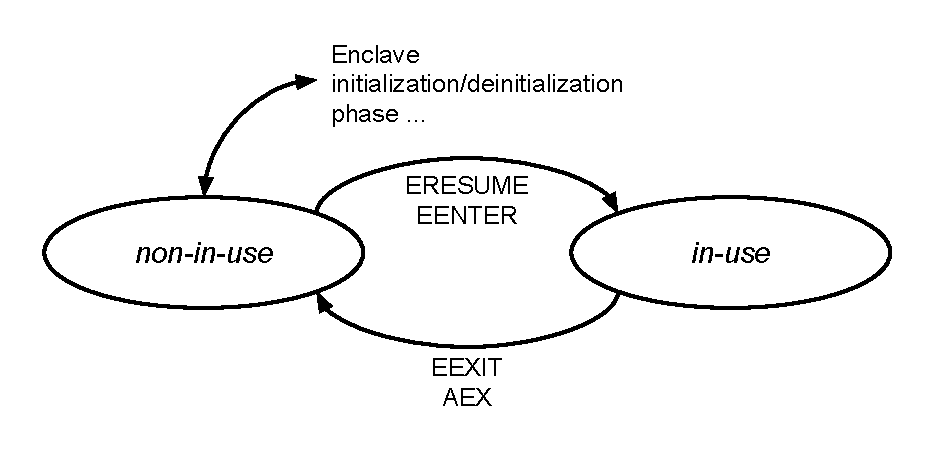
\includegraphics[width=0.6\textwidth]{fig_c6/fmi-standard}
	\caption[Standard SGX FSM.]{Standard Finite-State-Machine representation of 
	SGX Enclave~\citep{costan2016intel}.}
	\label{fig:fmi-standard}
\end{figure}

Due to SGX isolation properties, legitimate users cannot validate the runtime 
integrity of an 
enclave, which challenges their ability of identifying attack instances
effectively \citep{snakegx,biondo2018guard,lee2017hacking}.
To understand the underlying reason of this limit, we analyze the SGX 
enclave life-cycle, which is depicted as a Finite-State-Machine in 
Figure~\ref{fig:fmi-standard}.\footnote{This model is a simplified version 
of \cite{costan2016intel}.}
We assume the enclave has been loaded correctly and the host interacts with it 
by means of the opcodes described in Section~\ref{ssec:sgx-core-design}.
The model allows the enclave state to assume only two values: 
\emph{non-in-use} and \emph{in-use}.
In particular, an enclave transits to \emph{in-use} state when an 
\texttt{EENTER} or \texttt{ERESUME} is issued.
Then, the state returns to \emph{non-in-use} when an \texttt{EEXIT} or  
\texttt{AEX} happens.
This simple model is already implemented in the microcode: the same thread 
cannot enter (\ie \texttt{EENTER}) in an enclave which is 
already in \emph{in-use} state; it cannot exit (\ie \texttt{EEXIT}) when the 
enclave is in \emph{non-in-use}.

Intuitively, the model in Figure~\ref{fig:fmi-standard} provides limited
information about the enclave health. In case of new attacks against enclaves'
code~\citep{lee2017hacking,biondo2018guard,snakegx}, we are not able to
backtrace the enclave execution, and finally, distinguish whether an
enclave has been executed properly or not.
Moreover, current runtime RA works~\citep{abera2016c,aberadiat,scarr} focus 
only 
on stateless scenario, thus not fitting the enclaves needs.
SgxMonitor extends the standard SGX model in order to verify the correct 
enclaves runtime behavior, thus enhancing the SGX security guarantees.
%\todo{object}
%SGX enclaves are statful objects that can be modeled as a FSM,
%however, the standard FSM cannot represent modern \stbold{code-reuse attacks} 
%\newtxt{SGX attacks}
%(Section~\ref{sec:motivation}).
%\todo{options + challenge}
%\todo{our choose}
%On the contrary, SgxMonitor is the first runtime RA that employs an 
%enriched 
%FSM able to model the SGX enclaves and to capture modern attacks.
The SgxMonitor model is composed by four elements:
\begin{itemize}
	\item \emph{states}, that represent the runtime values of global structures	
	(Section~\ref{ssec:state}).
	\item \emph{actions}, that are meaningful binary level events (\eg 
	\texttt{EENTER}, function call) (Section~\ref{ssec:actions-definition}).
	\item graphs of \emph{actions}, that are computed offline and used to 
	validate runtime transactions (Section~\ref{ssec:graph-of-action}).
	\item \emph{transactions}, that are sequences of \emph{actions} leading an 
	enclave from a state to the next. They express correct execution paths 
	(Section~\ref{ssec:transaption-model}).
\end{itemize}
In the rest of the section, we detail state, \emph{actions}, transactions, and 
graphs of \emph{actions}. Finally, we show an example in 
Section~\ref{ssec:running-example}.

%\todo{FT: I feel like this paragraph should be removed.}
%The enclaves behavior depends by their internal state (\ie 
%global variables/structure), that  must be taken in account when we validate 
%the runtime correctness.
%Modern SGX code-reuse techniques target these structures for different 
%reasons: 
%Dark-ROP exploits anomalous exceptions handling to locate enclave gadgets, 
%Dilemma 
%forges specific structures to control the CPU registers.
%Tracing critical structures in our model allows an 
%external (trusted) entity to verify the enclave runtime state, and 
%finally reducing the attack surface.

\subsection{State Definition}
\label{ssec:state}

We define a state able to identify attacks that alter important global 
structures introduced by the Intel SGX SDK.
These structures handle operations such as \emph{outside function} 
invocation and \emph{exception handling} 
(Section~\ref{sec:software-guard-extension}), and are targeted by the 
adversaries~\citep{biondo2018guard,lee2017hacking}.
For instance, we can observe if an enclave is consuming a structure not 
previously generated, thus limiting the attack surface of 
modern threats~\citep{biondo2018guard,lee2017hacking}.

Due to the multi-threading nature of enclaves, SgxMonitor 
traces a state for each thread~\citep{intel-developer-guide}.
The state is a triplet defined as $(usage, structure, operation)$.
In particular, \emph{usage} recalls the FSM meaning seen in 
Figure~\ref{fig:fmi-standard} and can assume two values: \emph{in-use} and 
\emph{non-in-use}.
\emph{Structure}, instead, is an hash representation of the current structure 
used. If no \emph{structure} is used, it assumes \emph{null} value (\ie 
$\oslash$).
Finally, \emph{operation} represents the last operation performed over the 
\emph{structure}. In our model, the structures do not change over time, thus, 
we trace their generation (\ie G) and consumption (\ie C).
In case no operation has been performed, we consider a \emph{null} action (\ie 
$\oslash$).

In our proof of concept, we trace the generation and consumption of
\begin{enumerate*}[label=(\roman*)]
	\item \texttt{ocall\_context}, used in the \emph{outside 
		functions} invocation; and
	\item \texttt{sgx\_exception\_info\_t}, used in the 	
	\emph{exception handing}.
\end{enumerate*} 
These two structures are handled at thread granularity, thus they fit 
our model.
In Appendix~\ref{sec:model-examples_sgxmonitor}, we show their FSM 
representation.

%These structures handle high level operations such as \emph{outside functions} 
%invocation and exception handing 
%and the microcode does not validate their integrity.
%As a consequence, an adversary can tamper with them to control the 
%enclave execution
%Therefore, SgxMonitor embeds these structures to identify malicious 
%modifications.

\subsection{Action Definition}
\label{ssec:actions-definition}

Generally speaking, an \emph{action} is a meaningful software event.
We use the \emph{actions} to represent runtime enclave transactions
(Section~\ref{ssec:transaption-model}), that allow the evolution of the 
enclave state; and to build graph of \emph{actions} 
(Section~\ref{ssec:graph-of-action}), that we use to validate the runtime 
transactions.
In particular, we distinguish two type of \emph{actions}: \emph{generic} and 
\emph{stop}.

\paragraph{Generic actions.}
They identify standard software behaviors such as:
\begin{enumerate*}[label=(\roman*)]
	\item edges generated by \emph{control-flows} events; \eg \texttt{jmp}, 
	\texttt{call}, \texttt{ret};
	\item conditional branches (\eg \texttt{jc}); and
	\item function pointer and virtual table assignment.
\end{enumerate*}
Generic \emph{actions} do not alter the state of the enclave and they are 
used to identify correct executions.
We choose these events because they are key information to represent
execution paths~\citep{scarr,hu2018enforcing,kleen2015intel,7924286,9051250}.

\paragraph{Stop actions.}
They alter the state of the enclave, in particular, we consider particular SGX 
opcodes and structures manipulation.
For what concerns SGX opcodes, we consider \texttt{EENTER}, \texttt{EEXIT}, and 
\texttt{ERESUME}, moreover, we distinguish between \texttt{EEXIT} used for an 
ERET or an OCALL, respectively. These actions alter the first field of the 
state (\ie \emph{usage}): when an application enters an enclave, \emph{usage} 
becomes \emph{in-use}, while \emph{usage} turns to \emph{non-in-use} when the 
enclave exits.
For structures manipulations, instead, we trace whenever the enclave 
generates or consumes a structure. This actions alter the \emph{structure} and 
the	\emph{operation} fields in the state; \ie when an \emph{action} generates a 
structure, we store the new structure hash and set \emph{operation} as G, while 
we set \emph{structure} to null (\ie $\oslash$) and \emph{operation} to C when 
the structure gets consumed.

Both \emph{generic} and \emph{stop actions} are formalized as a triplet:
$$
a = (type, src, value)_{cond}.
$$
In particular, \emph{type} identifies the nature of the \emph{action} (\eg 
function call, \texttt{EENTER}).
\texttt{Src}, instead, is the virtual address at which the \emph{action} has 
been performed.
\emph{Value} depends by the actual \emph{action} semantic; for instance; it 
contains the \emph{callee} address in case of function call; a boolean value 
(\ie taken or not) in case of conditional branches; a \emph{null} \emph{value} 
(\ie $\oslash$) in case the \emph{action} does not require it.
Finally, \emph{cond} contains extra condition (\eg $value \ge 0$).
We provide the complete \emph{action} list in Table~\ref{tbl:actionss} grouped 
by \emph{generic} and \emph{stop}.


\begin{table}[t]
	\centering
	\begin{tabular}{ll}
		\toprule 
		\multicolumn{2}{l}{\textbf{Actions}} \\ \midrule
		\multicolumn{2}{l}{\emph{Generic}} \\ \midrule
		%		\textbf{Action} & {} \\ \midrule
		(E, \texttt{src}|$\oslash$, \texttt{dst}|$\oslash$) & Function 
		call, ind. jump, or ret inst. \\ 
		& \texttt{src} and \texttt{dst} can assume null value \\ 
		& (\ie $\oslash$) \\ %to implement a shadow stack \\
		(B, \texttt{src}, $0|1$) & Conditional branch \\
		& ($0$: not taken, $1$: taken) \\ 
		(A, \texttt{src}, \texttt{addr}) & Function pointer assignment \\ 
		(V, \texttt{src}, \texttt{vptr}) & Virtual pointer assignment \\
		& (for C++ virtual classes) \\ \midrule
		%		F & new frame generated when a function is invoked (to get local
		%		variables easier) \\
		\multicolumn{2}{l}{\emph{Stop}} \\ \midrule
		(G, \texttt{src}, \texttt{ctx}) & \texttt{ocall\_context} 
		generation  \\ 
		(C, \texttt{src}, \texttt{ctx}) & \texttt{ocall\_context} 
		consumption \\ 
		(J, \texttt{src}, \texttt{ctx}) & 
		\texttt{sgx\_exception\_info\_t} \\
		&  generation \\ 
		(K, \texttt{src}, \texttt{ctx}) & \texttt{sgx\_exception\_info\_t} \\
		& consumption \\ 
		(N, \texttt{src}, \texttt{idx}) & \texttt{EENTER} for the \emph{secure 
			function} \texttt{idx} \\ 
		(R, \texttt{src}, $\oslash$) & \texttt{ERESUME} \\ 
		(T, \texttt{src}, $\oslash$) & \texttt{EEXIT} from 
		\texttt{enter\_enclave} \\
		& (ERET) \\ 
		(D, \texttt{src}, $\oslash$) & \texttt{EEXIT} from \texttt{do\_ocall} \\
		& (OCALL) \\ 
		\bottomrule
	\end{tabular} 
	\caption[Valid transations definition.]{\emph{Actions} used to 
	define valid transactions grouped by \emph{generic} and \emph{stop}, 
	respectively.}
	\label{tbl:actionss}
\end{table}


\subsection{Graphs of Actions Definition}
\label{ssec:graph-of-action}

Graphs of \emph{actions} are composed by vertexes and edges.
More precisely, vertexes and \emph{actions} are in a bijective relationship, 
\ie each vertex is paired with exactly one \emph{action} and each \emph{action}
is paired with exactly one vertex.
The edges, instead, are combinations of \emph{actions} that appear at 
runtime.

We opted for graphs to efficiently represent loops, that otherwise require
an unpredictable sequence of \emph{actions}, we provide an example in
Section~\ref{ssec:running-example}.
Moreover, the graphs of \emph{actions} allow us to implement a shadow stack  
(further details in Section~\ref{sec:model-validation}).
Finally, we describe the algorithm to extract the graphs of \emph{actions} in 
Section~\ref{sec:model-exctraction}.
%, that identifies correct 
%edges while avoiding impossible ones (\ie symbolic execution excludes pairs of 
%\emph{actions} that do not appear at runtime).



\subsection{Transaction Definition}
\label{ssec:transaption-model}

A transaction identifies a valid execution path in an enclave and
is composed by a valid sequence of \emph{actions} 
(Section~\ref{ssec:actions-definition}) that makes the enclave state 
evolve.
%
%In our model, the state evolves through valid execution paths, that are 
%represented as sequence of \emph{actions} 
%(Section~\ref{ssec:actions-definition}). 
%The \emph{target enclave} T generates a stream of \emph{actions} during the 
%\emph{Online Enclave Verification}, that the \emph{Model Verifier} 
%(Section~\ref{sec:model-validation}) will validate aided by the graphs of 
%\emph{actions} (Section~\ref{ssec:graph-of-action}).
%Intuitively, the transition from a state to the next one happens only through
%valid transactions.
Formally, we indicate a transaction $P$ as following: 
$$
P = [g_1, \dots, g_n, s],
$$
which is a sequence of \emph{generic actions} $g_i$ that terminates with a 
\emph{stop action} $s$.
Intuitively, an enclave should reach a new state only through valid 
transactions, otherwise we observe an anomalous enclave behavior.
We perform the transaction validation by matching the \emph{actions} received
from the monitored enclave with its graphs of \emph{actions}.
We provide the full validation algorithm in Section~\ref{sec:model-validation}.

The \emph{actions} are traced by instrumenting the source code at compilation 
time (Section~\ref{ssec:compilation-unit}), moreover, we propose an 
efficient mechanism to transit the \emph{actions} in the presence of an 
adversarial host 
(Section~\ref{ssec:secure-communication-protocol}).
%Finally, we extract the valid execution paths through a combination of symbolic
% and static analysis (Section~\ref{sec:model-exctraction}).

%\todo{shall I remove this paragraph?}
%The standard SGX FSM contains only limited \emph{actions} (\eg 
%\texttt{EENTER}, 
%\texttt{EEXIT}) to define the state transaction, without considering the entire
%execution path traversed.
%However, code-reuse attacks allow an adversary to hijacks the victim execution 
%(\eg overwriting the return address),
%thus driving an enclave to valid state while keeping valid edge 
%\emph{actions}.

\subsection{Model Example}
\label{ssec:running-example}

\begin{figure}[t]
	\centering
	\begin{subfigure}[b]{0.45\textwidth}
		\centering
		\begin{lstlisting}[style=CStyle,escapechar=|,basicstyle=\ttfamily\tiny]
		struct state L;
		
		int fun(int a) {
		int x = 0;
		for (int i = 0; i < 10; i++) {
		traceBranch(1);
		traceEdge(16); // &add
		x += add(a, i);
		}
		traceBranch(0);
		traceEdge(__builtin_return_address(0));
		return x;
		}
		
		int add(int a, int b) {
		lock(L) // generates a new L
		int x = a + b;
		unlock(L) // consumes L
		traceEdge(__builtin_return_address(0));
		return x;
		}
		\end{lstlisting}
		\caption{The snipped of code used in our example.}
		\label{fig:running-example-code}
	\end{subfigure}
	\hfill
%	\\
	\begin{subfigure}[b]{0.45\textwidth}
		\centering
		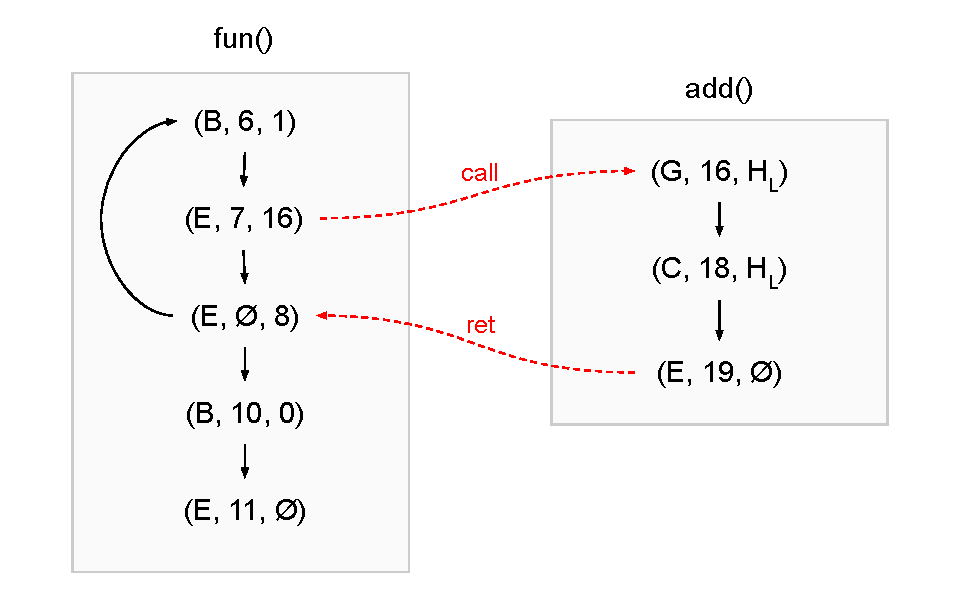
\includegraphics[width=\textwidth]{fig_c6/running-example-graph.pdf}
		\caption{The graphs of \emph{actions} used in our example.}
		\label{fig:running-example-graph}
	\end{subfigure}
	\caption[SgxMonitor running example.]{Snipped of code and relative graph of 
	\emph{actions} used to exemplify the SgxMonitor model. We use the graphs of 
	\emph{actions} to represent the internal behavior of the functions, and to 
	implement a shadow stack.}
	\label{fig:running-example}
\end{figure}

Figure~\ref{fig:running-example} shows an example of code and its graphs 
of \emph{actions}.

Figure~\ref{fig:running-example-code} contains a simple code that is composed 
by two functions \texttt{fun()} and \texttt{add()}, and a thread-bounded 
structure \texttt{L}.
We also add the tracing functions \texttt{traceBranch()} and 
\texttt{traceEdge()}, that emits the \emph{action} with type \texttt{B} 
(branch) and \texttt{E} (edge), respectively.
Finally, we assume that the function \texttt{lock()} and \texttt{unlock()} 
generates and consumes the structure \texttt{L}, respectively.
%\feedback{For sake of simplicity, we show a redundant instrumentation to show 
%each \emph{action} emitted.}
The tracing functions infer the \texttt{src} value from the 
stack, an attacker may attempt at tampering with the stack, but this will lead 
to an incorrect sequence of \emph{actions} that will be detected (more details 
in Section~\ref{ssec:secure-communication-protocol}).

Figure~\ref{fig:running-example-graph} shows the graphs of \emph{actions} 
relative to Figure~\ref{fig:running-example-code}.
Any vertex of the graphs represents a single \emph{action}, while the edges 
identify correct pairs of \emph{actions}.
The graphs enables us to describe the loop in \texttt{fun()}: $(\text{E}, 
\oslash, 8) \rightarrow (\text{B}, 6, 1)$.
We also detail few actions that are used to implement a shadow stack:
\begin{itemize}
	\item $(\text{E}, 7, 16)$ is the function call to the \texttt{add()} 
	function.
	
	\item $(\text{E}, \oslash, 8)$ is the return point from the \texttt{add()} 
	function. We indicate the \texttt{src} address as null (\ie $\oslash$) 
	because we do not know \emph{a-priori} the address of the return 
	instruction of \texttt{add()}.
	
	\item $(\text{E}, 19, \oslash)$ and $(\text{E}, 11, \oslash)$  are the exit 
	point of \texttt{add()} and \texttt{fun()} functions, respectively.
	We indicate the \texttt{dst} address as null (\ie $\oslash$) because we do 
	not know the caller.
\end{itemize}
%\todo{review this part}
We detail the validation algorithm in Section~\ref{sec:model-validation}.
In Appendix~\ref{sec:model-examples_sgxmonitor}, we describe the usage of our 
model for the \emph{outside function} invocation 
(Appendix~\ref{ssec:ocall-example}) and the exception handling 
(Appendix~\ref{ssec:exception-handling}).

\section{Design}
\label{sec:system-design_sgxmonitor}

\begin{figure}[t]
	\centering
		
    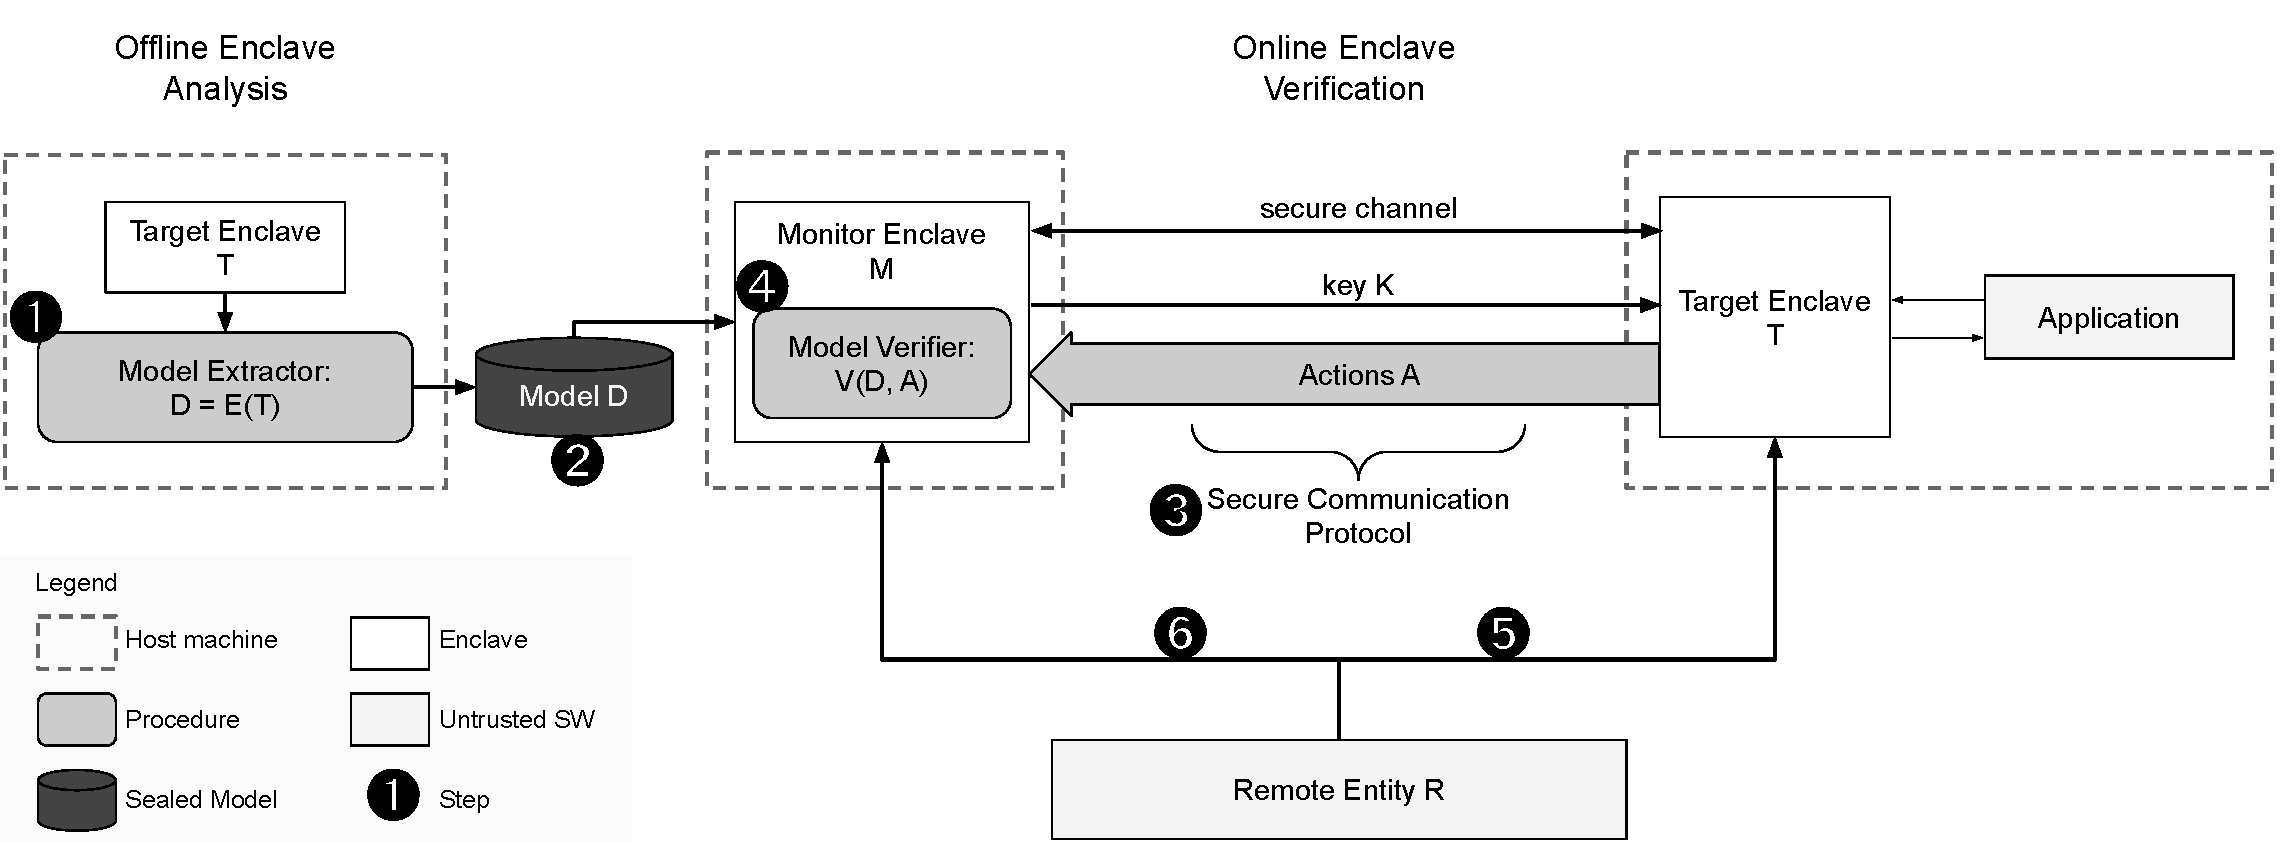
\includegraphics[width=\linewidth]{fig_c6/design.pdf}
    \caption[SgxMonitor design.]{The SgxMonitor design is composed by two 
    	distinct phases: Offline Enclave Analysis and Online Enclave 
    	Verification.
    	During the Offline Enclave Analysis, the \emph{Module Extractor} 
    	analyses 
    	the \emph{target enclave} T (\circled[1]) to obtain a \emph{Model} D 
    	that 
    	represents the correct behavior of T (\circled[2]).
    	During the Online Enclave Verification, an \emph{Application} 
    	interacts 	
    	with T by following standard SGX mechanisms (\eg ECALL, OCALL), 
    	meanwhile, 
    	T sends a stream of \emph{Actions} A to the \emph{monitor enclave} M 
    	through a \emph{secure communication protocol} (\circled[3]). 
    	M, then, uses a \emph{Model Verifier} to validate A against D 
    	(\circled[4]).
    	Finally, a \emph{remote entity} R can verify both the static software 
    	integrity of T through the standard SGX RA 							
    	protocol~\citep{anati2013innovative} (\circled[5]) and the runtime 
    	integrity of T by inquiring M about T runtime status (\circled[6]).}
    \label{fig:design_sgxmonitor}
\end{figure}


%\begin{figure}[t]
%	\centering
%	
%	\begin{adjustbox}{addcode={\begin{minipage}{\width}}{\caption[SgxMonitor 
%	design.]{%
%		The SgxMonitor design is composed by two distinct phases: 
%		Offline 
%		Enclave Analysis and Online Enclave Verification.
%		During the Offline Enclave Analysis, the \emph{Module Extractor} 
%		analyses
%		the \emph{target enclave} T (\circled[1]) to obtain a \emph{Model} D 
%		that 
%		represents the correct behavior of T (\circled[2]).
%		During the Online Enclave Verification, an \emph{Application} interacts 
%		with T by following standard SGX mechanisms (\eg ECALL, OCALL), 
%		meanwhile, 
%		T sends a stream of \emph{Actions} A to the \emph{monitor enclave} M 
%		through a \emph{secure communication protocol} (\circled[3]). 
%		M, then, uses a \emph{Model Verifier} to validate A against D 
%		(\circled[4]).
%		Finally, a \emph{remote entity} R can verify both the static software 
%		integrity of T through the standard SGX RA 	
%		protocol~\citep{anati2013innovative} (\circled[5]) and the runtime 
%		integrity of T by inquiring M about T runtime status (\circled[6]).}
%	\label{fig:design_sgxmonitor}\end{minipage}},rotate=90,center}
%	
%	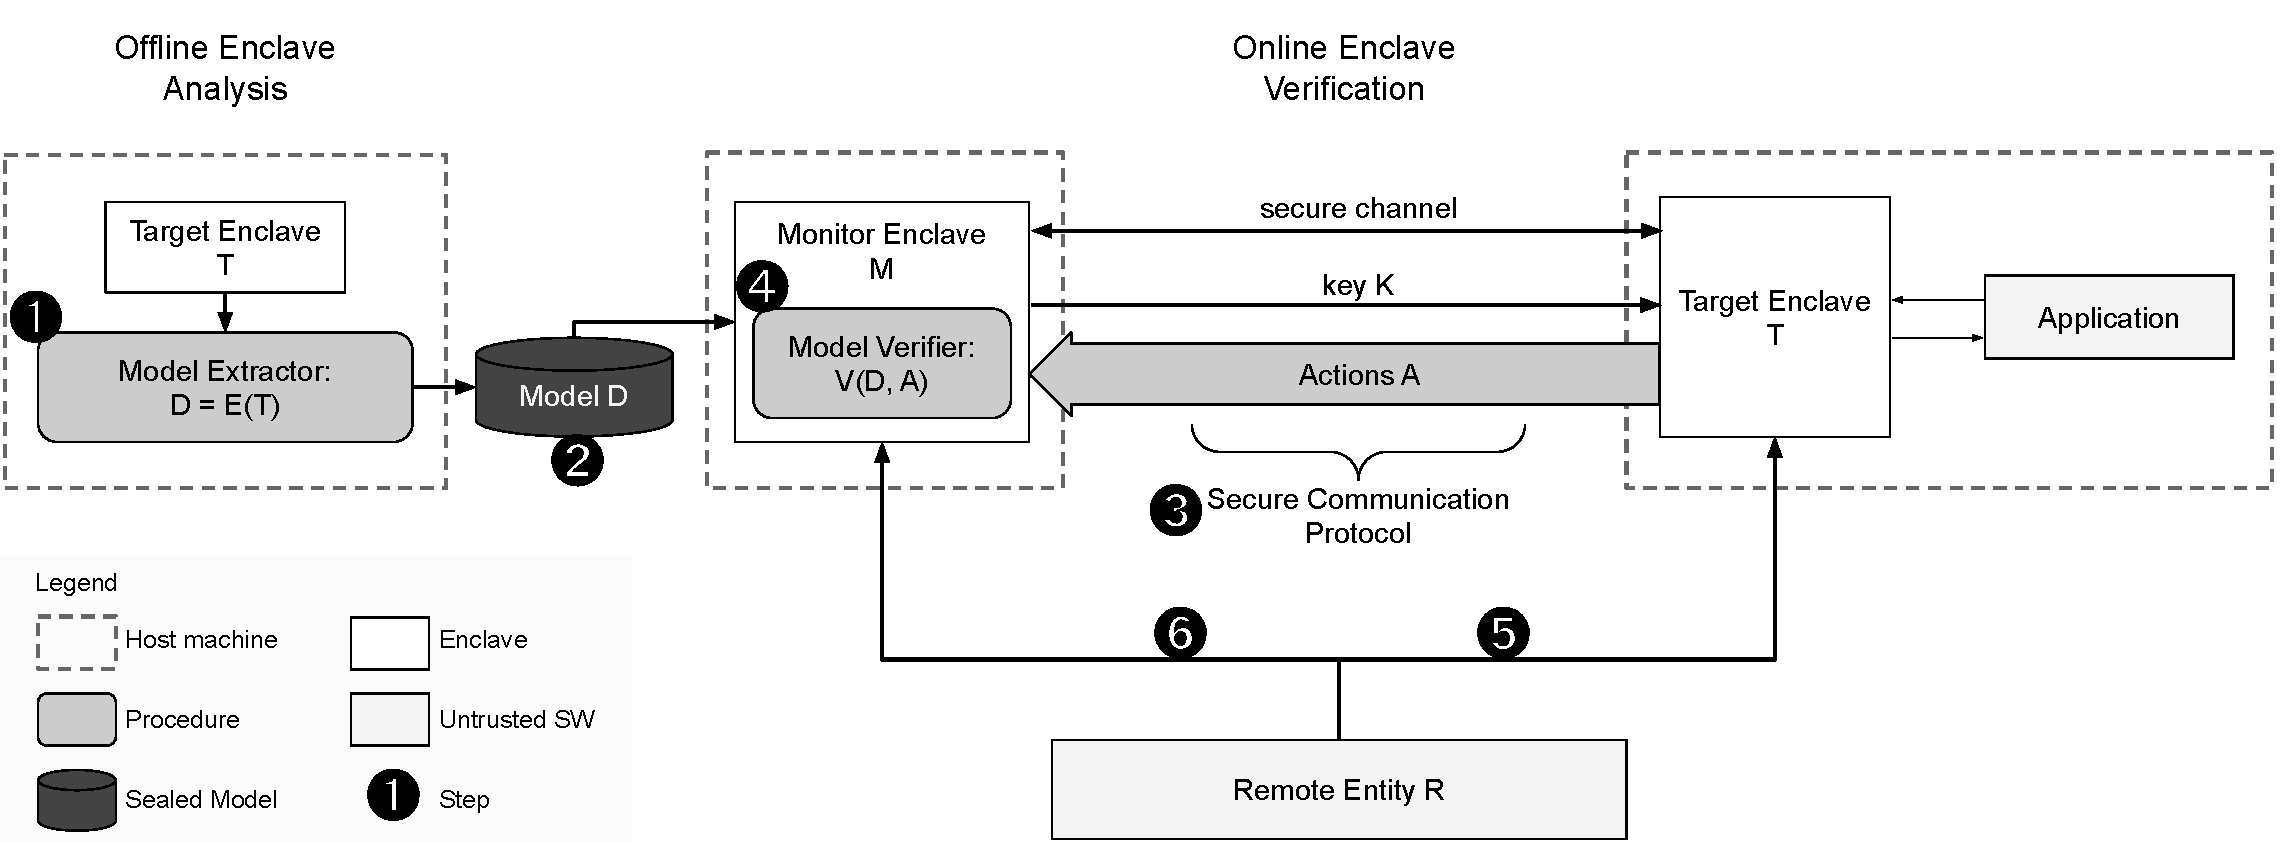
\includegraphics[width=\linewidth]{fig_c6/design.pdf}
%	\end{adjustbox}
%\end{figure}

Designing a runtime RA scheme that fits the SGX realm requires a re-thinking of 
standard approaches.
Classic runtime RA schemes assume having a protocol between two entities, 
called \emph{Prover} and \emph{Verifier}, respectively.
The \emph{Verifier} is considered trusted and outside of the attacker range, 
while the \emph{Prover} might be under attack. Moreover, the \emph{Prover} is 
equipped with a trusted anchor which is out of the 
attacker range as well (see Section~\ref{ssec:sgx-remote-attestation}).
In the SGX scenario, the \emph{Prover} is an enclave loaded in a 
malicious host, while the microcode (\ie CPU) plays the role of trusted anchor.
However, SGX has not been designed to validate the enclave runtime
properties. Moreover, we cannot observe the enclave behavior externally, \eg 
through Intel PT~\citep{kleen2015intel} or Intel 
LBR~\citep{7924286,9051250}.
In short, Intel did not design SGX to implement a runtime RA.
Considering the previous limitations, we propose a pure software design that 
implements a runtime RA for SGX enclaves.

To achieve the goal, we design a \emph{Prover} composed by two 
enclaves, namely \emph{target} and \emph{monitor}, respectively.
The \emph{target} enclave contains the actual \emph{secure functions}, 
communicates with the application, and can be compromised.
%\todo{FT: problem with assumptions: 1) the monitor host is 
%compromised -> then we have to ensure the monitor is not prone to memory 
%corruption errors; 2) the monitor host is trusted -> we do not need to use an 
%enclave as monitor; 3) if monitor host is compromised and monitor enclave is 
%error free -> we can put monitor and target in the same host.}
The \emph{monitor} enclave, instead, resides in a remote host out 
of the attacker range, and has the duty to validate the \emph{target} enclave 
runtime behavior.
Ideally, the \emph{target} enclave sends a stream of \emph{actions} to 
the \emph{monitor} that validates the \emph{target} integrity.
Thanks to this design, an external \emph{Verifier} can validate the runtime 
state of the \emph{target} by inquiring the \emph{monitor}.
%, it just needs to perform a standard RA with the monitor enclave, which
%can provide information about the target enclave state.
We provide an overview of our design in Section~\ref{ssec:overview}, and 
discuss other details in the rest of this section.
%sections~\ref{sec:model-exctraction}, \ref{sec:model_sgxmonitor}, 
%\ref{ssec:secure-communication-protocol}, and~\ref{sec:model-validation}.

\subsection{Overview}
\label{ssec:overview}
Figure~\ref{fig:design_sgxmonitor} illustrates the SgxMonitor design, that 
involves 
seven 
actors:
\begin{itemize}
	\item a \emph{target enclave} T, the enclave to protect against attacks 
	under the
	threat model described in Section~\ref{sec:threat-model_sgxmonitor}.
	\item a \emph{monitor enclave} M, that receives the \emph{actions} A 
	generated by T.
	\item an \emph{Application}, that interacts with T through standard SGX 
	specifications (\eg ECALL, OCALL),
	\item the \emph{Model} D, that represents the correct behavior of T.
	\item the \emph{Model Extractor}, that generates a model containing
	the correct behavior of T.
	\item the \emph{Model Verifier}, that validates the runtime status of T 
	according to A and D.
	\item a \emph{remote entity} R, that validates both software and runtime 
	integrity of T.
\end{itemize}

The design of SgxMonitor revolves around the model described in 
Section~\ref{sec:model_sgxmonitor}.
In particular, the SgxMonitor is split into two distinct phases: 
\emph{Offline 
	Enclave Analysis}, and \emph{Online Enclave Verification}. 
During the \emph{Offline Enclave Analysis}, the \emph{Model Extractor} 
implements the algorithms in Section~\ref{sec:model-exctraction} to extract the 
\emph{Model} D, that represents the correct behavior of the \emph{target 	
	enclave} T (\circled[1]).
Then, we seal D to prevent a malicious host to tamper with it (\circled[2]).
%\todo{while we describe our Model in Section~\ref{sec:model_sgxmonitor}}
During the \emph{Online Enclave Verification}, we assume that M and T are 
correctly loaded in the respective hosts.
Once T is loaded, it establishes a \emph{secure communication channel} with M 
by 
using the standard SGX RA~\citep{anati2013innovative}, as
described in Section~\ref{ssec:secure-communication-protocol} (\circled[3]).
This channel allows T to send a stream of \emph{Actions} A to M, 
while an \emph{Application} can interact with T by following standard SGX 
mechanisms (\eg ECALL, OCALL).
Finally, M uses the \emph{Model Verifier} to validate the runtime integrity 
of T by controlling A against D, as we describe in 
Section~\ref{sec:model-validation} (\circled[4]).
In the following sections, we detail each interaction described so far.

Once M correctly receives A from T, a \emph{remote entity} R can attest the 
software integrity of T through the standard SGX RA~\citep{anati2013innovative} 
(see Section~\ref{ssec:sgx-remote-attestation}). This ensures that the software 
in T has been loaded properly and is not tampered  (\circled[5]).
Since we employ the standard SGX RA, we do not provide further details.
Finally, R can validate the runtime integrity of T through a simple query 
toward M, which returns the runtime status of T, \ie \emph{trusted} or 
\emph{untrusted} (\circled[6]).


\subsection{Model Extractor}
\label{sec:model-exctraction}

\begin{algorithm}[t]
	\SetAlgoLined
	\DontPrintSemicolon
	\SetKwFunction{algo}{extractModel}
	\SetKwProg{myalg}{}{}{}
	\myalg{\algo{T}}{
		$m \gets \emptyset$\;
		\For{$f \in T.\text{instr\_functions}$}{ \label{alg:model-extractor-for}
			setSymbolicGlobalVars($T$)\; \label{alg:model-extractor-glb}
			loopAnalysis($f$)\; \label{alg:model-extractor-loop}
			setSymbolicFreeArgs($f$)\; \label{alg:model-extractor-free}
			$r \gets \text{symbolicExploration}(f)$\;			
			\label{alg:model-extractor-symex}
			\If{$r.\text{isTimeout}()$} {
				$r \gets \text{insensitiveAnalysis}(f)$\; 
				\label{alg:model-extractor-ins}
			}
			$m \gets m \cup (f, r.\text{graph\_of\_action})$\; 
			\label{alg:model-extractor-mod}
		}
		\Return $m$
	}
	\caption{Extracting model algorithm, it takes as input the target enclave 
		and returns the relative model.}
	\label{alg:model-extractor}
\end{algorithm}

The goal of the \emph{Model Extractor} is to automatically infer the 
behavior for a given enclave. A naive approach would use a symbolic 
execution~\citep{king1976symbolic} over the entire enclave.
However, this strategy does not scale for the whole code base.
Another approach would use insensitive static 
analysis~\citep{coppa2017rethinking} to extract the control-flow graphs of each 
function. However, this approach introduces impossible paths that increases the 
attacker surface.
In our scenario, we assume that the code in an enclave is not as 
complex as generic software~\citep{abadi2009control} (\eg a web-browser).
An enclave contains a relative small number of indirect call and its 
software base is given.
Therefore, we take inspiration from previous compositional 
analysis~\citep{calcagno2009compositional} that treats individual functions 
separately.
More precisely, we extract a graph of \emph{actions} for each function of the 
enclave with a combination of symbolic executions and insensitive static 
analysis.

The \emph{Model Extractor} takes as input a \emph{target enclave} T which has 
been instrumented at compilation time (Section~\ref{ssec:compilation-unit});
\ie it contains extra code that traces the \emph{actions} described in 
Section~\ref{sec:model_sgxmonitor}; and outputs a graph of \emph{actions} for 
each traced 
function in the enclave.
%The graphs of \emph{actions} are an important component our model and allow us 
%to validate the runtime behavior of T.
T is compiled without debug information, we solely rely on global symbols to 
identify the functions entry point and the global variables.
The global symbols do not contribute to the enclave measurement, thus we strip 
them out after extracting the model~\citep{rozas2013intel} 
(Section~\ref{ssec:sgx-remote-attestation}). 

Overall, the extraction algorithm is described in 
Algorithm~\ref{alg:model-extractor}. Given an instrumented \emph{target 
	enclave} T, we analyze each instrumented function separately 
(Alg.~\ref{alg:model-extractor} line~\ref{alg:model-extractor-for}).
We describe each point of the analysis in the rest of the section, while we 
formalize the model in Section~\ref{sec:model_sgxmonitor}.

\paragraph{Symbolic Global Variables (Alg.~\ref{alg:model-extractor} 
	line~\ref{alg:model-extractor-glb}).} 
Global variables might contain default concrete values that affect the symbolic 
exploration.
We mitigate this issues by setting all the global variables as unconstrained
symbolic objects. 
We repeat this operation for each function to clean the symbolic constraints 
previously set. 

\paragraph{Loop Analysis (Alg.~\ref{alg:model-extractor} 
	line~\ref{alg:model-extractor-loop}).}

%\todo{riporta un po' ovunque}
%\todo{object}
Unbounded loops can lead to infinite symbolic 
explorations~\citep{10.1007/978-3-642-36742-7_47}.
%\todo{options + challenge} ?? ok
%\todo{assumptions}
%\todo{scelta}
Since we are interested to reduce false positive alarms, we employed a 
postdomination tree~\citep{dominators} over the static control-flow-graph to 
identify the loops header in each function.
This approach is conservative and allows us to explore more execution paths, 
which is our main goal.
We set a three maximum loop interaction similarly to previous 
works~\citep{wang2009intscope}.
Our experiments show that we reach a good coverage while keeping low false 
positive.

\paragraph{Free Arguments Inferring (Alg.~\ref{alg:model-extractor} 
	line~\ref{alg:model-extractor-free}).}
%\todo{say backward slicing, conservative. Point to analysis. Intra-procedural. 
%Program dependence graph.}
Some function requires pointers as arguments (\eg structures, objects, array), 
however, current symbolic explorations do not fully handle symbolic 
pointers, that might lead to a wrong or incomplete 
exploration~\citep{coppa2017rethinking}.
Since we are interested to reduce false positive alarms, we opted for a 
conservative approach based on static backward slicing~\citep{slicing}
to identify pointers passed as function arguments.
For each free pointer, we build an unconstrained symbolic object to help 
the exploration.
%This algorithm is not meant to resolve all the possible cases, such as 
%aliasing, contexts or callbacks.
This solution allows us to achieve a good coverage in 
the majority of the case, as also shown in our experiments. We also 
introduce custom analysis to handle corner cases, which are though a 
limited number.
Finally, we deal with functions pointers by employing a conservative function 
type analysis~\citep{abadi2009control}.

\paragraph{Symbolic Exploration (Alg.~\ref{alg:model-extractor} 
	line~\ref{alg:model-extractor-symex}).}
We primary employ a symbolic exploration~\citep{king1976symbolic} to avoid 
impossible paths that, otherwise, might increase the attacker surface.
We execute the symbolic exploration after tuning the function as previously 
described.
Through the exploration, we build the graph of \emph{actions} for each 
function. 

\paragraph{Insensitive Static Analysis (Alg.~\ref{alg:model-extractor} 	
	line~\ref{alg:model-extractor-ins}).}
Since few functions of our use case experienced a symbolic execution timeout 
due to their complexity (\ie too many nested loops).
We employed a fallback approach based on an insensitive static 
analysis~\citep{sarkar2007flow} in which we traverse the static 
control-flow-graph of the function to build the graph of \emph{actions}.
These cases are rare and they are used only if the symbolic approach fails.
We measure the frequency of this case in our evaluation.

\paragraph{Building a Model (Alg.~\ref{alg:model-extractor} 	
	line~\ref{alg:model-extractor-mod}).}
The output is an association between functions and relative graph of 
\emph{actions}.
We use the latter to compose the model (Section~\ref{sec:model_sgxmonitor}) and 
to 
validate the correct enclave behavior (Section~\ref{sec:model-validation}).
Finally, we seal the output in the \emph{monitor enclave} host to avoid 
tampering.

\subsection{Secure Communication Protocol}
\label{ssec:secure-communication-protocol}

T and M exchange messages relying on a secure communication channel resilient 
against an adversarial host that may alter, eavesdrop, or forge the packets.

\paragraph{Protocol properties.}
Our protocol ensures two properties:
\begin{enumerate*}[label=(\roman*)]
	\item the host cannot tamper with the packets emitted by T;
	\item an adversary cannot alter or forge the packets already emitted even 
	if she takes control of T.
\end{enumerate*}
Note that we accept an adversary that performs a denial-of-service between T 
and M.
In this case, M considers T as untrusted after a timeout.

\paragraph{Attacks before protocol establishing.} 
Issuing the protocol requires the \emph{Application} to invoke a dedicated 
secure function of T before being able to use the its other secure functions.
We insert additional checks that ensure no other 
functionality of T is active until T and M successfully established the channel.
This design avoids an adversary to attack T before M starts monitoring it.

\paragraph{Workflow.}
The channel requires three steps to be established (\circled[3] in 
Figure~\ref{fig:design_sgxmonitor}):
\begin{enumerate*}[label=(\roman*)]
	\item T issues a standard SGX RA~\citep{anati2013innovative} with M, thus 
	ensuring a respective identity verification;
	\item M sends a secure \emph{key} K to T; and
	\item T sends the \emph{actions} to M.
\end{enumerate*}
The secure channel is shared among the threads of T, that refer to the same 
key K.
We also include a thread ID into the exchanged packets, this allows M and T to 
multiplex and demultiplex the communication.
The adoption of a shared key K avoids an adversary to use 
the technique discussed in Dark-ROP~\citep{lee2017hacking}, we provide more 
details in the next paragraphs.

The validation of the transmitted \emph{actions} relies on two algorithms, 
\texttt{emitLog()} and \texttt{verifyLog()}, that are illustrated in the
algorithms~\ref{alg:emit-log} and~\ref{alg:verify-log}, respectively.
Both \texttt{emitLog()} and \texttt{verifyLog()} use a lock to avoid
concurrency problems.
Finally, K has the same size of the packets transmitted, thus avoiding 
crypto-analysis~\citep{horstmeyer2013physical}.

T emits a new action $A$ through instrumented code.
$A$ is given as an input to \texttt{emitLog()} that encrypts and transfers it 
to M over an insecure channel.
First,  \texttt{emitLog()} creates a \emph{mac} by using an hash function $H$ 
and the concatenation of $A$ and the key K (Line~\ref{alg:emit-log:1}  
Alg.~\ref{alg:emit-log}).
Then, it generates $C$ by \emph{xor}-ing the concatenation of \emph{action} $A$ 
and \emph{mac} with the key K (Line~\ref{alg:emit-log:2} 
Alg.~\ref{alg:emit-log}).
At this point, it generates a new key K by hashing the 
current key K (Line~\ref{alg:emit-log:3} Alg.~\ref{alg:emit-log}).
Finally, the function writes $C$ into an insecure channel 
(Line~\ref{alg:emit-log:4} Alg.~\ref{alg:emit-log}).

On the other side, M relies on \texttt{verifyLog()} to decrypt and validate the 
encrypted packets $C$.
We also assume that M receives the packets in 
order.\footnote{We assume a reliable channel like TCP as in \cite{scarr}.}
First, M decrypts the pair $(A|\text{mac})$ by \emph{xor}-ing the packet $C$ 
and the key K (Line~\ref{alg:verify-log:1} Alg.~\ref{alg:verify-log}).
Then, M verifies the correctness of the packet received by independently 
computing \emph{mac}$^\prime$ (Line~\ref{alg:verify-log:2} 
Alg.~\ref{alg:verify-log}).
If \emph{mac} and \emph{mac}$^\prime$ does not agree, $C$ was tampered during 
the transmission and M sets T as untrusted (Line~\ref{alg:verify-log:4} 
Alg.~\ref{alg:verify-log}).
Otherwise, $A$ is considered correct and is processed as described in 
Section~\ref{sec:model-validation} (Line~\ref{alg:verify-log:5}  
Alg.~\ref{alg:verify-log}).
Finally, M generates the next key K similarly to T 
(Line~\ref{alg:verify-log:6} Alg.~\ref{alg:verify-log}).

\paragraph{Defense against a tampered enclave T}
Our protocol can resist against an adversary that exploits T.
In this case, the adversary may abuse a memory corruption error to 
diverge the enclave execution path.
However, we instrument the code of T such that it emits the \emph{action} 
before the enclave traverses the hijacked edge.
Therefore, the \emph{action} results already encrypted and shipped, while K has 
been altered by the hashed function.
We face three scenarios here:
\begin{enumerate*}[label=(S\arabic*)]
	\item the compromised \emph{action} reaches M, thus letting the
	latter to recognize the attack;
	\item the host drops the \emph{action} before reaching M, thus letting the 
	latter to recognize the attack after a timeout; and
	\item the adversary attempts to forge a new valid \emph{action}, however, 
	she cannot retrieve K after \texttt{emitLog()} invocation (\ie a new K is 
	produced).
\end{enumerate*}
In all these cases, M will observe an anomaly in the protocol or T 
behavior, finally setting T as untrusted.

Sharing the same key K among the threads defeats the tactic described 
in modern enclave attacks~\citep{lee2017hacking}.
In their scenario, an \emph{adversary} exploits a thread
to leak information (\ie the key K) from another thread.
In our design, leaking K forces a thread to emit an \emph{action} X 
representing the attack. Moreover, \texttt{emit()} ensures the \emph{actions} 
follows a specific order. 
Therefore, either X reaches M, thus revealing the attack; or X is 
dropped, thus showing an anomaly.

\begin{algorithm}[t]
	\SetAlgoLined
	\DontPrintSemicolon
	\SetKwFunction{algo}{emitLog}
	\SetKwProg{myalg}{}{}{}
	\myalg{\algo{A}}{
		$\text{mac} \gets H(A|K)$\; \label{alg:emit-log:1}		
		$C \gets (A|\text{mac}) \oplus K$\; \label{alg:emit-log:2}
		$K \gets H(K)$\; \label{alg:emit-log:3}
		$write(C)$\; \label{alg:emit-log:4}
	}
	\caption{Procedure used by the \emph{target} enclave to emit logs in a  
		secure fashion.}
	\label{alg:emit-log}
\end{algorithm}
\begin{algorithm}[t]
	\SetAlgoLined
	\DontPrintSemicolon
	\SetKwFunction{algo}{verifyLog}
	\SetKwProg{myalg}{}{}{}
	\myalg{\algo{C}}{
		$(A|\text{mac}) \gets C \oplus K$\; \label{alg:verify-log:1}
		$\text{mac}^\prime \gets H(A|K)$\; \label{alg:verify-log:2}
		\eIf{$\text{mac}^\prime \neq \text{mac}$} {\label{alg:verify-log:3}
			$\text{untrusted}()$\; \label{alg:verify-log:4}
		}{
			$\text{process}(A)$\; \label{alg:verify-log:5}
		}
		$K \gets H(K)$\; \label{alg:verify-log:6}
	}
	\caption{Algorithm used by the \emph{monitor} enclave to verify the 
		logs 
		emitted through \emph{emitLog()} described in 		
		Algorithm~\ref{alg:emit-log}.}
	\label{alg:verify-log}
\end{algorithm}


\subsection{Model Verifier}
\label{sec:model-validation}

The \emph{Model Verifier} receives a stream of \emph{actions} from the 
\emph{target enclave} T.
Our validation algorithm ensures that the received \emph{actions} match the 
\emph{Model} D. 
Moreover, we implement a \emph{remote shadow stack} to ensure a correct 
function invocation and to handle recursions~\citep{scarr}.
To explain the validation, we recall the example illustrated in  
Figure~\ref{fig:running-example}.
Moreover, we assume the \emph{Model Verifier} receives a 
stream of \emph{actions} that can be split in three transactions as follow:
\begin{align*}
P_1 &= (\text{B}, 6, 1) \rightarrow (\text{E}, 7, 16) \rightarrow (\text{G}, 
16, H_L),\\
P_2 &= (\text{C}, 18, H_L),\\
P_3 &= (\text{E}, 19, 8) \rightarrow (\text{B}, 6, 1) \rightarrow (\text{E}, 7, 
16) \rightarrow (\text{G}, 16, H_L).
\end{align*}
The transactions $P_1$, $P_2$, and $P_3$ adhere to the definition in
Section~\ref{ssec:transaption-model}, \ie they are a sequence of \emph{generic 
	actions} (\ie type B and E) that terminates with a \emph{stop} one (\ie 
	type G 
and C). 
We also consider as a valid transaction $P_2$, which does not contain 
\emph{generic actions}.

%In a real scenario, the shadowstack contains the function traversed in the 
%rRts 
%to reach \texttt{secure\_function()}.
%Here, however, we consider an empty shadow stack for sake of simplicity.
At the beginning, we assume a \emph{Model Verifier} with an initial state as 
$(\emph{in-usage}, \oslash, \oslash)$ because the control is already in the 
enclave but no structure has been used yet.
Moreover, we assume an empty \emph{shadow stack}, that we indicate as $[]$.
In this case, the \emph{Model Verifier} uses the graph of \emph{actions} of 
\texttt{fun()} and tries to match it with the transaction $P_1$.
The first \emph{action} of $P_1$ is $(\text{B}, 16, 1)$, that is the 
for-loop entrance.
%Then, we observe $(\text{E}, 7, 16)$ and recognizes a function call to 
%\texttt{add()} due to the \texttt{dst} 
%address; 
Then, we observe $(\text{E}, 7, 16)$, that represents a function call to 
\texttt{add()} due to the \texttt{dst} address; 
\ie the first instruction of the \texttt{add()} function is at line $16$.
At this point, we do two operations:
\begin{enumerate*}[label=(\roman*)]
	\item push into the \emph{shadow stack} the pair $(\texttt{fun}, (\text{E}, 
	\oslash, 8))$, whose second element is the first instruction to execute 
	once \texttt{add()} returns (see Figure~\ref{fig:running-example-graph}); 
	and 
	\item use the graph of \emph{actions} of \texttt{add()} to validate further 
	\emph{actions}.
\end{enumerate*}
In particular, a new frame $(\texttt{fun}, (\text{E}, \oslash, 8))$ is pushed 
into the \emph{shadow stack} as follow:
$$
[] \rightarrow [(\texttt{fun}, (\text{E}, \oslash, 8))].
$$
Next, we observe $(\text{G}, 16, H_L)$, which is a \emph{stop action} that 
terminates $P_1$.
$(\text{G}, 16, H_L)$ also generates a new value of \texttt{L}, thus altering 
the enclave state as follow:
$$
(\emph{in-usage}, \oslash, \oslash) \rightarrow (\emph{in-usage}, H_L, G).
$$

Now, the \emph{Model Verifier} receives $P_2$ and observes only $(\text{C}, 18, 
H_L)$, that consumes the previous structure generated and alters the states as 
follow:
$$
(\emph{in-usage}, H_L, G) \rightarrow (\emph{in-usage}, \oslash, C).
$$
If $P_2$ contained a different \emph{stop action}, \eg $(\text{C}, 18, H_X)$, 
the \emph{Model Verifier} would notice that $H_X \neq H_L$, thus recognizing 
an attempt of T to consume (\ie restore) a wrong structure. As consequence 
of such discrepancy, T will turn untrusted.

The last transaction $P_3$ is processed. The \emph{Model Verifier} 
observes $(\text{E}, 19, 8)$, that is the combination of $(\text{E}, \oslash, 
8)$, already in the \emph{shadow stack}, and $(\text{E}, 19, \oslash)$, which 
is the 
last \emph{action} for \texttt{add()} (see 
Figure~\ref{fig:running-example-graph}).
It, thus, compares the \texttt{src} and \texttt{dst} addresses
of the runtime action $(\text{E}, 19, 8)$ with the two \emph{actions} 
$(\text{E}, \oslash, 8)$ and $(\text{E}, 19, \oslash)$.
This ensures that \texttt{add()} is returning to the correct location, and 
the frame $(\texttt{fun}, (\text{E}, \oslash, 8))$ is popped out the 
\emph{shadow stack} as follows:
$$
[(\texttt{fun}, (\text{E}, \oslash, 8))] \rightarrow [].
$$
In case the return address is corrupted, the \emph{shadow stack} does not 
match, 
\eg we receive $(\text{E}, 19, X)$ that differs from $(\text{E}, \oslash, 8)$,
as a consequence, the \emph{Model Verifier} sets T as untrusted.
The remaining \emph{actions} of $P_3$ lead again through the for-loop and follow
the same verification phase.
%Finally, the \emph{action} $(\text{B}, 8, 0)$ matches the next 

\section{Implementation}
\label{sec:implementation}

Here, we provide technical details about SgxMonitor implementation: the 
\emph{Compilation Unit} 
(Section~\ref{ssec:compilation-unit}), the \emph{Model 
	Extractor} (Section~\ref{ssec:model-generation}), and the 
\emph{secure communication channel} (Section~\ref{ssec:monitor-target-channel}).

\subsection{Compilation Unit}
\label{ssec:compilation-unit}

The \emph{Compilation Unit} takes as input the \emph{target enclave} source code
and emits the instrumented enclave T.
The unit is implemented as an LLVM pass for the version $9$ (367 LoC) and a 
modified version of Clang $10$ that instruments virtual pointer assignments (15 
LoC added).
In the link phase, we link T with an instrumented SGX SDK to trace specific 
parts of the code, \eg
in \texttt{do\_ocall} and \texttt{asm\_oret} to handle 
\texttt{ocall\_context} generation/consumption; and \texttt{enter\_enclave}
to trace the entrance/exit from the enclave.
We opted for this solution because Intel does not officially support the 
compilation of the SGX SDK with Clang~\citep{sgxclang}.
We based the instrumented SGX SDK on the version $2.6$.

In this process, we also include an extra secure function that issues the 
\emph{secure communication channel}, and extra checks that avoid the 
interaction between T and the \emph{Application} before the channel is 
established (see Section~\ref{ssec:secure-communication-protocol}).


\subsection{Model Extractor}
\label{ssec:model-generation}

The \emph{Model Extractor} is based on angr version $8.18$ and implements the 
algorithms described in Section~\ref{sec:model-exctraction}.
We use PyVex~\citep{shoshitaishvili2015firmalice}, the intermediate 
representation of angr, to navigate the static CFG of the 
functions, and angr symbolic engine to extract the graphs of \emph{actions}.
The \emph{Model Extractor} is composed by $8416$ LoC in total.

%\begin{itemize}
%	\item[X] Instrumentation: LLVM pass on v9.0.0.
%	\item[X] Clan version 10.0.0 modified to trace vptr assignment
%	\item[X] Angr Version: 8.19.10.30 from pip
%	\item[X] SGX SDK version 2.6
%\end{itemize}


%\begin{figure}[t]
%	\centering
%	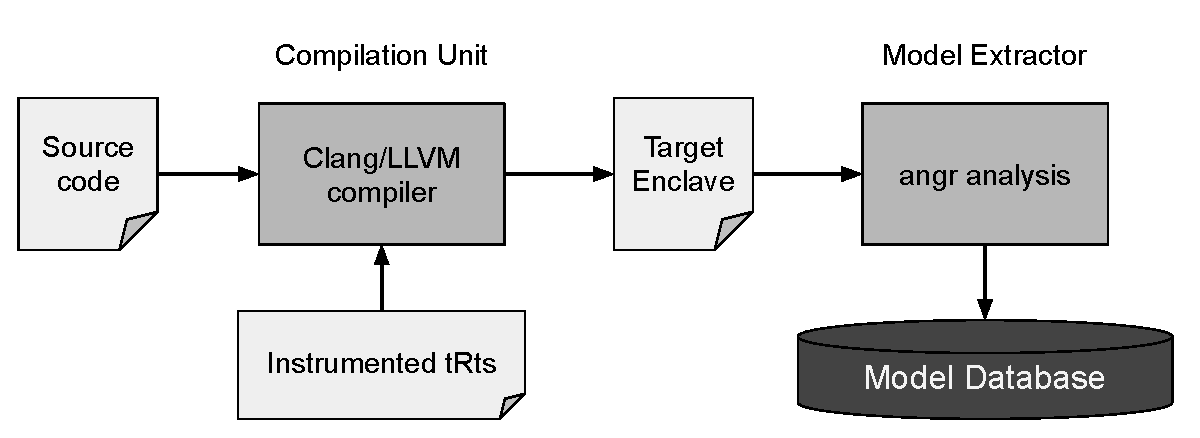
\includegraphics[width=0.9\linewidth]{fig_c6/model-generator.pdf}
%	\caption{SgxMonitor model generator architecture.}
%	\label{fig:model-generator}
%\end{figure}

\subsection{Secure Communication Channel}
\label{ssec:monitor-target-channel}

The communication between the \emph{target enclave} T and the \emph{monitor 
	enclave} M is implemented by combining a TCP connection and a switchless 
mechanism~\citep{tian2018switchless}.
T writes encrypted actions (see 
Section~\ref{ssec:secure-communication-protocol}) into a ring-buffer that 
resides in the untrusted host.
The buffer is then flushed into a TCP socket that connects T and M.
On the M side, another ring-buffer feeds the \emph{Module Verifier}.
We employ this design to reduce context switch 
delays~\citep{tian2018switchless}.

To implement the functions \texttt{emitLog()} and \texttt{verifyLog()}, we use
the \emph{sha256} implementation provided by Intel SGX SDK.
We can improve the efficiency adopting other
secure functions such as the Intel SHA extension~\citep{gulley2013intel} or 
Blake2~\citep{aumasson2013blake2}.

%- I use a TCP socket + switchless to reduce context-switch delay.

%- I use sha256 as hash function, in future it is possible to use the hardware 
%version

\section{Evaluation}
\label{sec:evaluation}

We design our evaluation following the guidelines described 
in~\citep{van2019sok} to avoid benchmarking flaws.
Our evaluation revolves around two main questions:
\begin{enumerate*}[label=(\textbf{RQ\arabic*})]
	\item can I use SgxMonitor in a \emph{real scenario}?
	\item \emph{what} and \emph{how} can SgxMonitor protect me?
\end{enumerate*}
We answer \textbf{RQ1} in Section~\ref{ssec:usage-evaluation}.
More precisely, we measure micro-benchmark, macro-benchmark, attestation speed, 
coverage and precision.
We answer \textbf{RQ2} in Section~\ref{ssec:security-properties} by testing 
the SgxMonitor security guarantees against a set of modern SGX attacks.

\subsection{RQ1 - Usage Evaluation}
\label{ssec:usage-evaluation}

We describe the use cases used, the experiment setup, and discuss the 
impact of SgxMonitor in real projects.

\paragraph{Use Cases.}
We identified $10$ open-source projects that use SGX. 
Most of them do not compile because they refer to old SGX 
features or they are incompatible with Clang.
Among them, we choose five use cases:
\begin{enumerate*}[label=(\roman*)]
	\item \textsf{Contact}~\citep{signalrepo}, the contact discovery service 
	used 
	by Signal app~\citep{signalapp} ($4138$ LoC and $6$ secure functions); 
	\item an SGX porting of \textsf{libdvdcss}~\citep{libdvdcss}, a portable 
	DRM 
	algorithm used by VLC media player~\citep{videolan} ($3438$ LoC and $4$ 
	secure functions); 
	\item \textsf{StealthDB}~\citep{stealthdb}, a 
	PostgreSQL~\citep{momjian2001postgresql} plugin that uses SGX to encrypt
	tables ($10351$ LoC and $3$ secure functions);
	\item \textsf{SGX-Biniax2}~\citep{bauman2016case}, an SGX poring of the 
	open-source game Biniax2~\citep{biniax2} ($4696$ LoC and $7$ secure 	
	functions); and
	\item a \textsf{unit-test} to validate corner cases of the enclave 
	behaviors not covered previously, like 
	exception handling ($583$ LoC and $3$ secure functions).
\end{enumerate*}
We use \textsf{Contact}, \textsf{StealthDB}, \textsf{SGX-Biniax2}, and the 
\textsf{unit-test} to stress micro-benchmarks 
(Section~\ref{ssec:microbenchmark}) and attestation speed 
(Section~\ref{ssec:attesation-speed}).
We use \textsf{libdvdcss}, \textsf{StealthDB}, and \textsf{SGX-Biniax2} for 
macro-benchmarks (Section~\ref{sssec:macro-benchmar}).
All the five use cases are used for coverage and precision analysis 
(Section~\ref{sssec:coverage}).

\paragraph{Experiment Setup.}
All the experiments were performed on a Linux machine with kernel version 
$4.15.0$ and equipped with an Intel i7 processor and $16$GB of memory.
We set the CPU power governor as \emph{power save}.
Moreover, we perform a warm-up round for each \emph{secure function} before 
actually recording the performances.

\begin{figure}[t]
	\centering
	%	\begin{subfigure}{.33\textwidth}
	%		\centering
	%		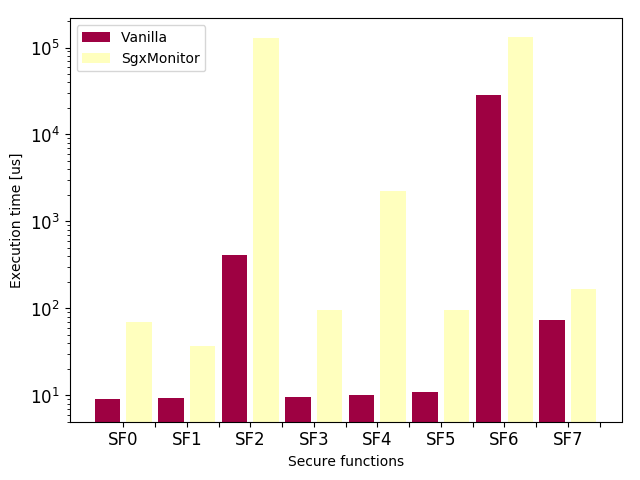
\includegraphics[width=\linewidth]{fig_c6/overhead.png}
	%		\caption{microbenchmark of secure functions with and without 
	%		SgxMonitor active.}
	%		\label{fig:overhead}
	%	\end{subfigure}
	%	~
	\begin{subfigure}[t]{.47\textwidth}
		\centering
		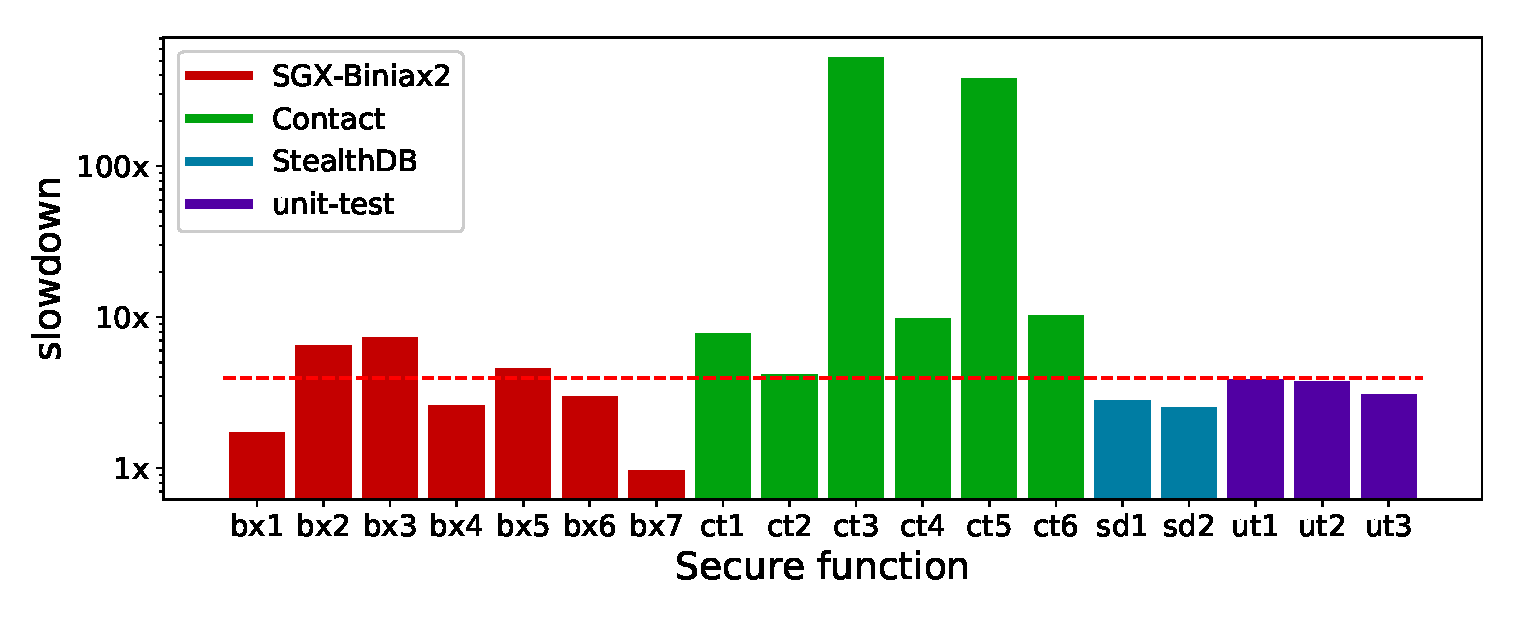
\includegraphics[width=\linewidth]{fig_c6/multiply.eps}
		\caption{Overhead of vanilla secure functions versus SgxMonitor 
			secure 
			functions of \textsf{Contact} (ct\emph{x}), \textsf{SGX-Biniax2} 
			(bx\emph{x}), \textsf{StealthDB} (sd\emph{x}) and 
			\textsf{unit-test} enclave (ut\emph{x}) expressed in logarithmic 
			scale. Median overhead is around $3.9$x and is depicted as a dashed 
			line.}
		\label{fig:multiply}
	\end{subfigure}
	\hfill
	\begin{subfigure}[t]{.47\textwidth}
		\centering
		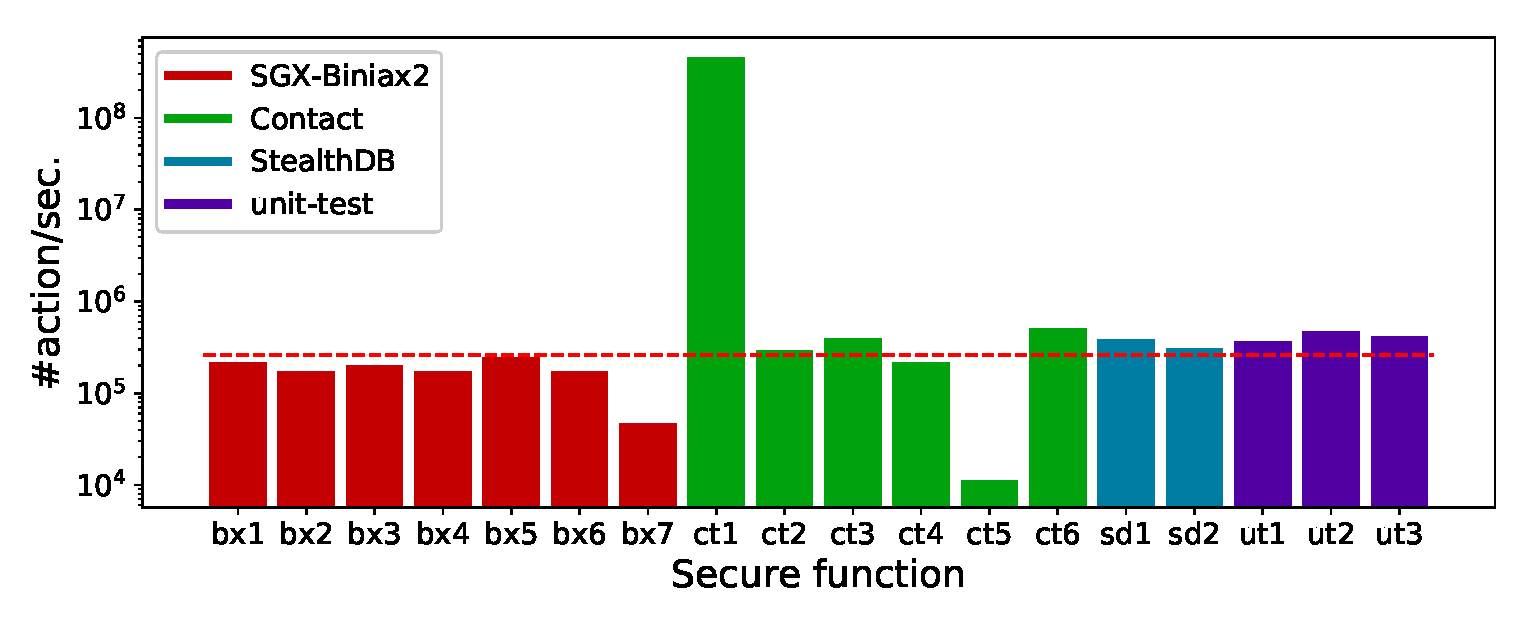
\includegraphics[width=\linewidth]{fig_c6/action-second.eps}
		\caption{Number of \emph{actions} processed per second of 
			\textsf{Contact} (ct\emph{x}), \textsf{SGX-Biniax2} 
			(bx\emph{x}), \textsf{StealthDB} (sd\emph{x}) and 
			\textsf{unit-test} enclave (ut\emph{x}). Median value is $260$K 
			\emph{action} per second and is depicted as a dashed line.}
		\label{fig:action-second}
	\end{subfigure}
	\caption{SgxMonitor micro-benchmark and \emph{action} speed measurement 
		evaluation.}
	\label{fig:fig}
\end{figure}

\subsubsection{Micro-benchmark}
\label{ssec:microbenchmark}

In this experiment, we measure the overhead of the single secure functions
with SgxMonitor and without (\ie vanilla).
We perform this experiment on \textsf{Contact}, \textsf{SGX-Biniax2}, 
\textsf{StealthDB} and the \textsf{unit-test} enclave.
The results are shown in Figure~\ref{fig:multiply}.
%, more precisely, ct\emph{x} indicates the results of the \textsf{Contact} 
%secure functions and ut\emph{x} of the \textsf{unit-test} ones.
In most of the cases, SgxMonitor introduces an overhead less than or equal 
to 
$10$x (bx$1$-$7$, ct$1$-$2$, ct$4$, ct$6$, ut$1$-$3$) with a median overhead of 
$3.9$x.
Only two secure functions show an overhead over $100$x (ct$3$ and ct$5$).

\vspace{0.5cm}
\noindent \textbf{Micro-benchmark---Take Away.}
A major source of overhead is incurred by the hash functions in the secure 
communication protocol (Section~\ref{ssec:secure-communication-protocol}), as 
observed in previous runtime RA~\citep{scarr,abera2016c,aberadiat}.
Different hash functions can ease the overhead, \eg the Intel SHA 
extension~\citep{gulley2013intel} or Blake2~\citep{aumasson2013blake2}.
However, This result does not really affect the performance of SgxMonitor 
that is line with previous works~\citep{scarr} for the of attestation speed 
(Section~\ref{ssec:attesation-speed}) and final user experience 
(Section~\ref{sssec:macro-benchmar}).

%\todo{OLD discussion, shall we keep it?}
%We analyzed the discrepancy between ct$3$ and ct$5$ and other secure 
%functions by observing the composition of the secure function execution 
%(\emph{t}),
%which is composed by the context switch delay (\emph{cs}) and an actual 
%execution time delay (\emph{ex}): $t = cs + ex$.
%In all the cases, the contribution of \emph{cs} is constant due to the 
%warm-up that smoothed random machine status (\eg cache, microcode delay) while
%\emph{ex} depends on the number of \emph{actions} emitted.
%Overall, all the functions, but ct$3$ and ct$5$, emit a similar number of 
%\emph{actions} thus the contribution of \emph{ex} is similar.
%On the contrary, ct$3$ and ct$5$ emit a higher number of \emph{actions}, thus 
%the contribution of \emph{ex} impacts more compared with the \emph{cs} one.

%We discuss a macrobenchmark analysis to measure whether the micro-level 
%overhead might afflict the final user experience 
%(Section~\ref{sssec:macro-benchmar}).

\subsubsection{Attestation Speed}
\label{ssec:attesation-speed}

Figure~\ref{fig:action-second} measures the attestation speed in terms of 
number of \emph{actions} emitted and validated per second (on the y-axes) for 
each \emph{secure functions} of \textsf{Contact}, \textsf{SGX-Biniax2}, 
\textsf{StealthDB}, and the \textsf{unit-test} enclave (on the x-axes).
The execution time encompasses the context-switch delay, \emph{actions} 
emission, transmission, and verification at the \emph{monitor} side.

All the secure functions, but ct$1$, ct$5$ and bx$7$, express a throughput
that ranges from $167$K \emph{action}/sec (bx$2$) to $496$K 
\emph{action}/sec (ct$6$), with a median value of $260$K \emph{action}/sec.

\vspace{0.5cm}
\noindent \textbf{Attestation Speed---Take Away.}
These figures are in line with the previous RA works \citep{scarr}.
ct$1$, instead, emits a fewer number of  \emph{actions} and biases the 
attestation speed.
Finally, bx$7$ and ct$5$ perform sealing operations \citep{anati2013innovative} 
and thus introduce an extra delay per \emph{action}.

%ut1 :    357827.7105449074
%ut2 :    463019.3737053735
%ut3 :    408761.67014568264
%ct1 : 441153737.0238829
%ct2 :    282257.30575993075
%ct3 :    387111.21562789154
%ct4 :    208793.78303779676
%ct5 :     10860.764002950118 -> slower?
%ct6 :    496361.2341876099
%bx1 :    208324.6531394525
%bx2 :    167192.47488478257
%bx3 :    193815.88874967984
%bx4 :    169665.373libdvdcss61086474
%bx5 :    238251.72527111403
%bx6 :    167479.25118165914
%bx7 :     46067.869091001514
%sd2 :    300232.68032725365
%sd1 :    377292.38812606956

\begin{figure}[t]
	\centering
	\begin{subfigure}[b]{0.49\textwidth}
		\centering
		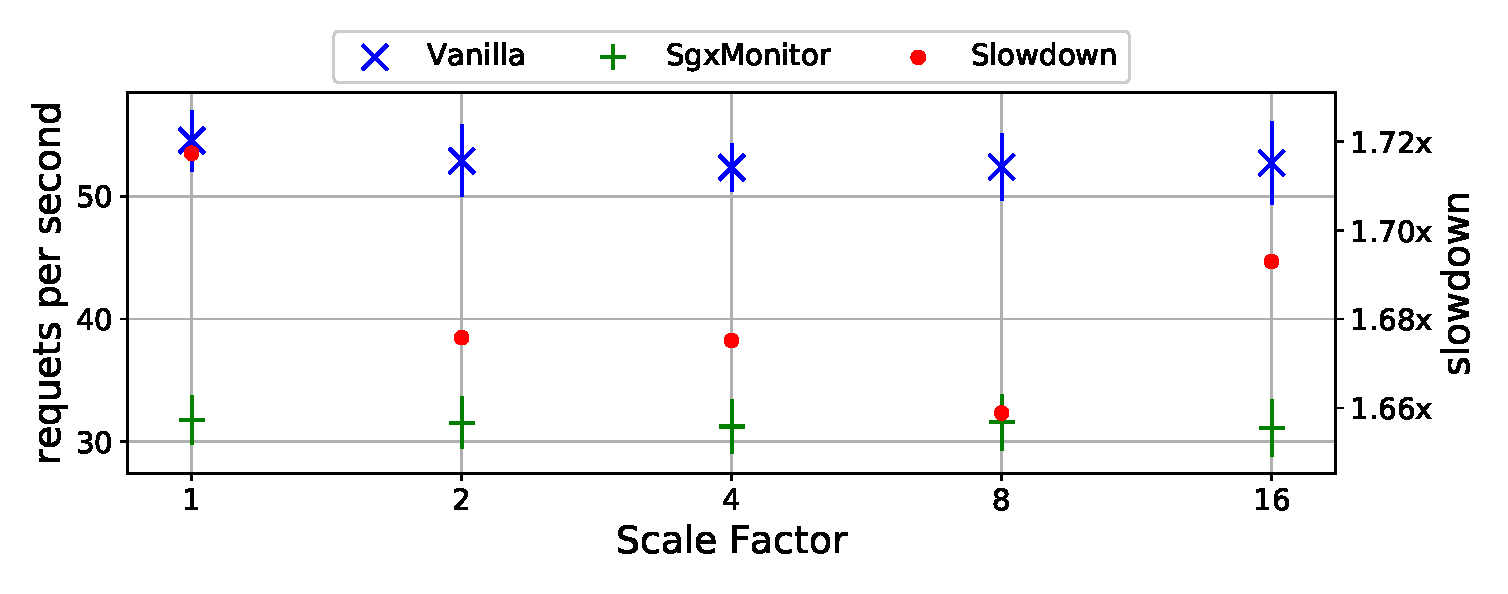
\includegraphics[width=\textwidth]{fig_c6/request_per_second.eps}
		\caption{Overhead of \textsf{StealthDB} vanilla and with SgxMonitor 
			measured as requests per second.
			Overall, SgxMonitor introduces an average slowdown of $1.68$x with 
			a 
			standard deviation of $0.02$x.}
		\label{fig:request_per_second}
	\end{subfigure}
	\hfill
	\begin{subfigure}[b]{0.49\textwidth}
		\centering
		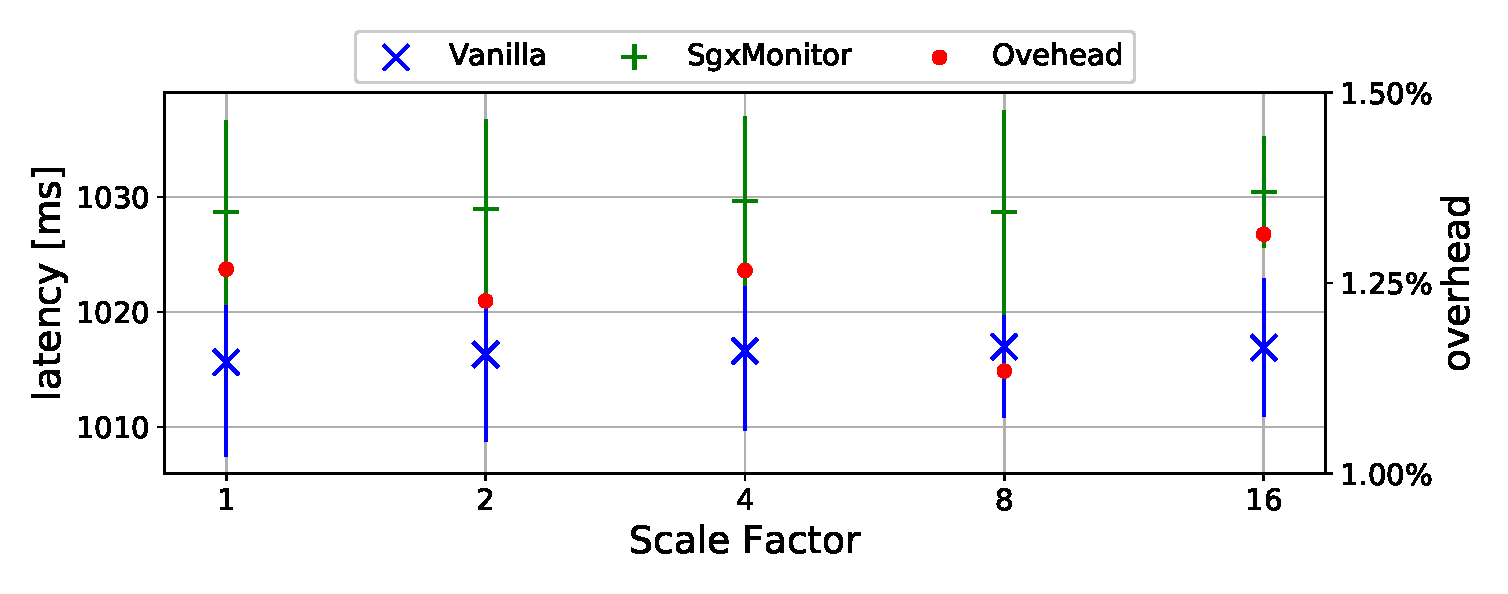
\includegraphics[width=\textwidth]{fig_c6/latency_2.eps}
		\caption{Overhead of \textsf{StealthDB} vanilla and with SgxMonitor 
			measured as latency (ms). 
			Overall, SgxMonitor introduces an average overhead of $1.24$\% with 
			a  
			standard deviation of $0.06$\%.}
		\label{fig:latency_2}
	\end{subfigure}
	\caption[SgxMonitor \textsf{StealthDB} 
	macro-benchmark.]{\textsf{StealthDB}~\citep{stealthdb} 
	performances measured against OLTP~\citep{oltp} benchmark and expressed as 
	request per second and latency. We evaluated \textsf{StealthDB} vanilla and 
	with SgxMonitor, in particular, we run $10$ measurements for each scale 
	factor (from $1$ to $16$) and plot average and standard deviation for 
	requests per second and latency, respectively.}
	\label{fig:request_per_second_latency}
\end{figure}

\begin{figure}[t]
	\centering
	\begin{subfigure}[t]{0.49\textwidth}
		\centering
		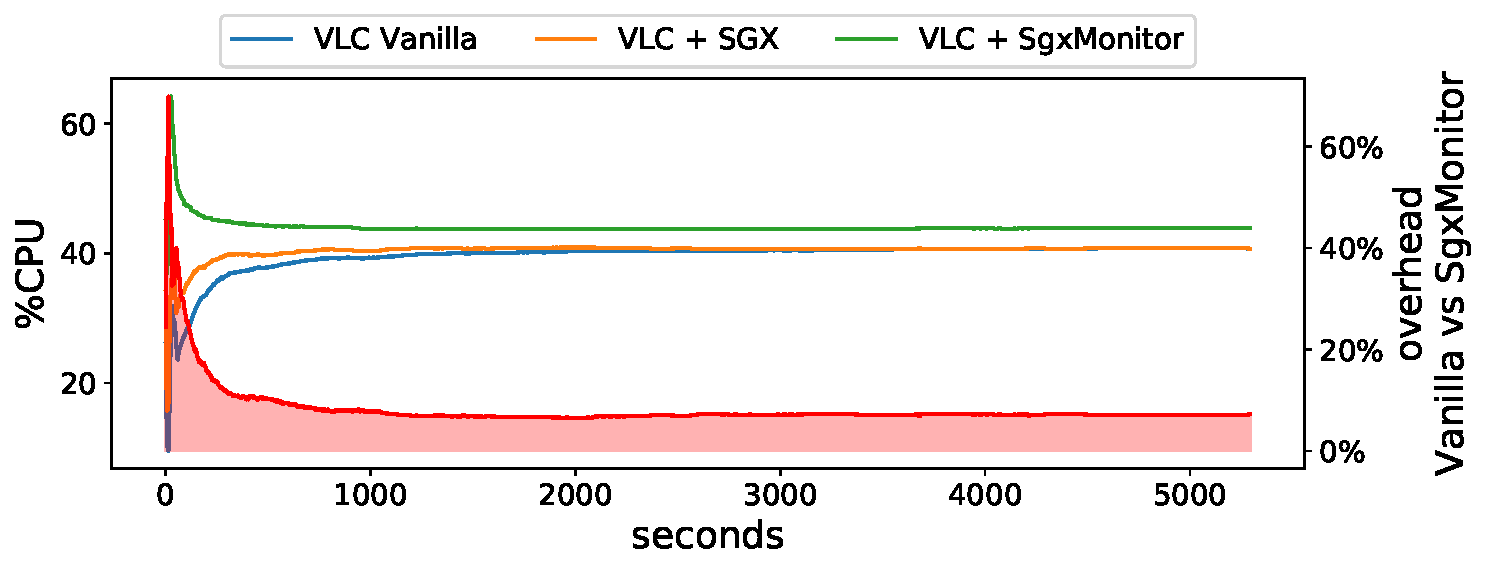
\includegraphics[width=\textwidth]{fig_c6/vlc_performance.pdf}
		\caption{Overhead of VLC with \textsf{libdvdcss} vanilla, plus SGX, and 
			plus SgxMonitor, respectively. We measure the percentage of CPU 
			usage 
			while playing the same DVD with the three settings.
			After an initial adjusting phase, the overhead drops and reaches a 
			plateau lower then $10$\%.}
		\label{fig:vlc_performance}
	\end{subfigure}
	\hfill
	\begin{subfigure}[t]{0.49\textwidth}
		\centering
		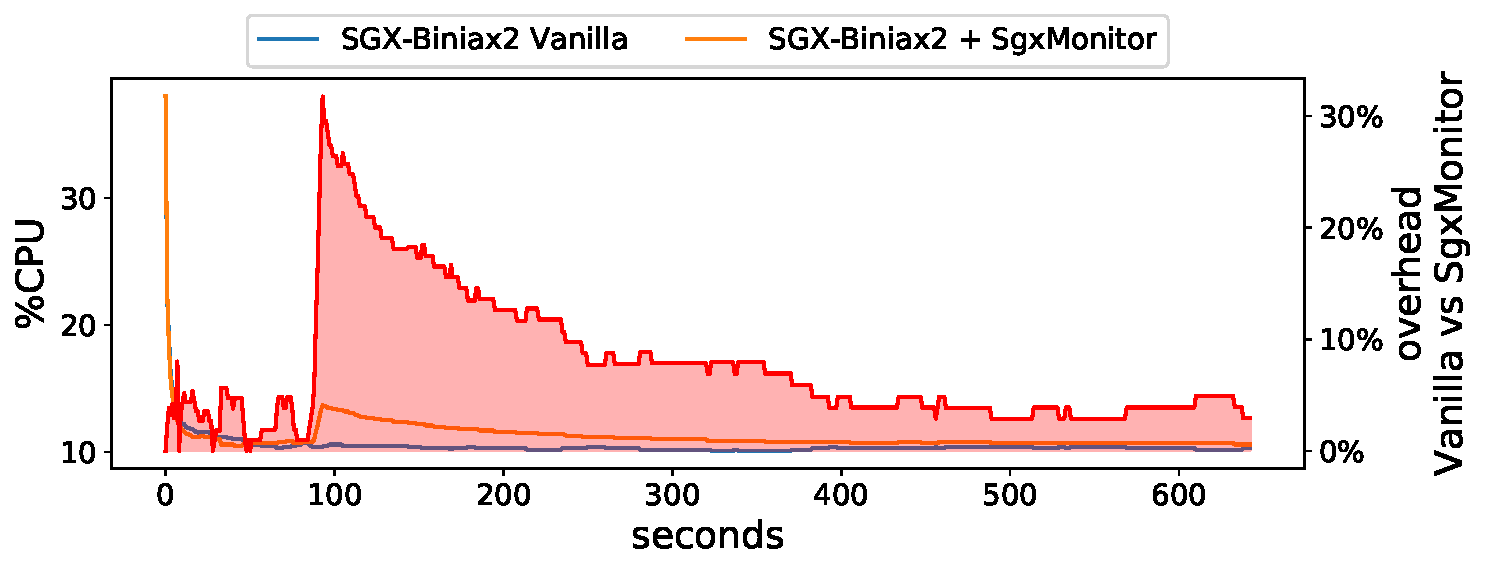
\includegraphics[width=\textwidth]{fig_c6/biniax2_performance.pdf}
		\caption{Overhead of \textsf{SGX-Biniax2} vanilla and with 
			SgxMonitor, 
			respectively. We measure the percentage of CPU usage while playing 
			the 
			game for the same amount of time (around $20$m).
			After an initial adjusting phase, the overhead drops and reaches a  
			plateau at around $5$\%.}
		\label{fig:biniax2_performance}
	\end{subfigure}
	\caption[SgxMonitor \textsf{libdvdcss} and \textsf{SGX-Biniax2}
	macro-benchmark.]{Macro-benchmark of \textsf{libdvdcss}~\citep{libdvdcss}, 
	deployed over VLC media player~\citep{videolan}, and 		
	\textsf{SGX-Biniax2}~\citep{bauman2016case}. In both cases, we measured the 
	CPU usage and the overhead introduced by SgxMonitor versus the vanilla 
	version of the software.}
	\label{fig:vlc_biniax2_performance}
\end{figure}

\subsubsection{Macro-benchmark}
\label{sssec:macro-benchmar}

We investigate the impact of SgxMonitor in three real applications.
\begin{enumerate*}[label=(A\arabic*)]
	\item \textsf{StealthDB} \citep{stealthdb}, which is a plugin for 
	PostgreSQL \citep{momjian2001postgresql} based on SGX.
	\item \textsf{libdvdcss} \citep{libdvdcss}, which is a DRM library used in 
	VLC media player \citep{videolan}.
	\item \textsf{SGX-Biniax2} \citep{bauman2016case}, which is an SGX porting 
	of the open-source game Biniax2 \citep{biniax2}.
\end{enumerate*}

\paragraph{StealthDB.}
We replicated the same experiments described in the 
original paper~\citep{stealthdb}. 
In particular, we deployed \textsf{StealthDB} over a 
PostgreSQL~\citep{momjian2001postgresql} version $10.15$ 
and we run the database benchmarking tool OLTP~\citep{oltp} by using the
five scale factors indicated in the original work.
Then, we reported the requests per second and the latency in 
figure~\ref{fig:request_per_second} and~\ref{fig:latency_2}, respectively.
For each scale factor, we run $10$ experiments and indicate average and 
standard deviation.
Overall, SgxMonitor introduces an average slowdown of $1.68$x and an 
overhead 
of $1.25\%$ in terms of requests per second and latency, respectively.

\paragraph{libdvdcss.}
We measured the CPU impact of SgxMonitor over \textsf{libdvdcss}, which is 
an 
DRM library used in VLC media player~\citep{videolan}.
For the experiment, we used a VLC version $3.0.8$, on which we deployed three 
versions of \textsf{libdvdcss}~\citep{libdvdcss}: vanilla, with SGX, and with 
SgxMonitor.
During the experiment, we played a DVD for around one hour and half while 
sampling the CPU usage every second.
Figure~\ref{fig:vlc_performance} shows the result of our experiment, after a 
first adjusting phase, the overhead reaches a plateau below $10\%$.
Furthermore, we did not experience any delay or interruption while playing the 
DVD in any of the three configurations.

%\vspace{2.5mm}
\paragraph{SGX-Biniax2.}
We measured the CPU impact of SgxMonitor over 
\textsf{SGX-Biniax2}~\citep{bauman2016case}, an example of video game porting 
that uses SGX for data protection.
In particular, we played the game for around $20$ minutes and we sampled the 
CPU usage every second.
Figure~\ref{fig:biniax2_performance} shows the result of our experiment, 
similarly to \textsf{libdvdcss}, we observed a first adjusting phase followed 
by a plateau at around $5\%$.
Furthermore, we did not experience any delay or interruption while playing 
\text{SGX-Biniax2} in any of the two configurations.

\vspace{0.5cm}
\noindent \textbf{Macro-benchmark---Take Away.}
The results of our experiments show that the overhead introduced by 
SgxMonitor is overall limited, \eg the slowdown in \textsf{StealthDB} is lower 
than the micro-benchmarks (\ie $1.6$x vs $3.9$x) and the CPU overhead expressed 
by \textsf{libdvdcss} and \textsf{SGX-Biniax2} shows a limited plateau.
Therefore, we conclude that SgxMonitor does not affect the final user 
experience and can be included into projects that either require occasional 
enclave interactions (like DRM protection) or are more computational intense 
(like a database).


%\begin{table}[t]
%	\centering
%	\begin{tabular}{lrrrr}
%		\toprule 
%		& \multicolumn{2}{c}{\emph{csstest}} & \multicolumn{2}{c}{VLC} \\
%		& \multicolumn{1}{c}{SgxMon.} & \multicolumn{1}{c}{vanilla} & 
%		\multicolumn{1}{c}{SgxMon.} & \multicolumn{1}{c}{vanilla} \\ \midrule
%		user [s]   & $0.260$ & $0.020$ & $34.660$ & $11.420$ \\ 
%		system [s] & $0.020$ & $0.020$ & $0.890$ & $2.210$ \\
%		total [s]  & $0.278$ & $0.315$ & $30.484$ & $30.635$ \\
%		CPU load   & $100\%$ & $12\%$ & $120\%$ & $44\%$ \\
%		\bottomrule
%	\end{tabular} 
%	\caption{Macrobenchmark of SgxMonitor implemented in \textsf{libdvdcss} 
%and 
%	deployed on \emph{ccstest} and VLC. Overall, the CPU load and the kernel is 
%	more involved because SgxMonitor requires a dedicated thread that 
%	costantely sends \emph{actions} to a \emph{monitor}. During the 
%	experiments, we did not observe any lag playing the DVD.\todo{replace with 
%	VLC, SGX-Biniax, and StealthDB plots}}
%	\label{tbl:macrobenchmark}
%\end{table}


\begin{table}[t]
%\begin{sidewaystable}
	\centering
	\resizebox{\columnwidth}{!}{%
	\begin{tabular}{lrrrrrrrrrr}
		\toprule 
		
		\multirow{2}{*}{Use case} &
		\multirow{2}{*}{\# functions} & 
		\multicolumn{2}{c}{\emph{action}} & 
		\multicolumn{2}{c}{edge} & 
		\multicolumn{1}{c}{\% \emph{action}} & 
		\multicolumn{1}{c}{\# functions} & 
		\multicolumn{3}{c}{analysis time [s]} \\ 
		
		& & \multicolumn{1}{c}{$\mu$} & \multicolumn{1}{c}{$\sigma$} & 
		\multicolumn{1}{c}{$\mu$} & \multicolumn{1}{c}{$\sigma$} & 
		\multicolumn{1}{c}{explored} & \multicolumn{1}{c}{static} & 
		\multicolumn{1}{c}{$\mu$} & \multicolumn{1}{c}{$\sigma$} & 
		\multicolumn{1}{c}{total} \\
		
		\midrule	
		\textsf{Contact} & $71$ & $12.77$ & $12.59$ & $15.09$ 
		& 
		$17.64$ & $96.4\%$ & $1$ & $20.20$ & $85.9$ & $1397.12$ \\
		\textsf{libdvdcss} & $47$ & $25.40$ & $22.05$ & 
		$34.44$ 
		& $31.50$ & $92.8\%$ & $8$ & $93.44$ & $205.3$ & $4205.18$ \\
		\textsf{StealthDB} & $44$ & $18.29$ & $13.53$ & 
		$21.97$ & $18.05$ & $96.6\%$ & $0$ & $6.16$ & $24.5$ & $258.89$ \\
		\textsf{SGX-Biniax2} & $49$ & $8.55$ & 
		$8.75$ & $9.29$ & $11.71$ & $91.6\%$ & $4$ & $52.46$ & $168.8$ & 
		$2465.62$ \\
		\textsf{Unit-test} & $17$ & $6.88$ & $7.47$ & $7.17$ & $10.52$ & 
		$94.0\%$ & $0$ & $15.60$ & $53.4$ & $234.29$ \\ 
		\midrule
		\emph{total} & $228$ & - & - & - & - & - & $13$ & - & - & $8561.10$ \\ 
		\bottomrule
	\end{tabular}%
	}
	\caption[Coverage analysis of SgxMonitor.]
		{Coverage analysis over our five use cases: 
		\textsf{Contact}~\citep{signalrepo}, 	
		\textsf{libdvdcss}~\citep{libdvdcss}, 
		\textsf{StealthDB}~\citep{stealthdb}, 
		\textsf{SGX-Biniax2}~\citep{bauman2016case}, and a unit-test. The 
		results show that the analysis covers from $91.6\%$ to $96.6\%$ of the 
		\emph{actions} in around $2$ hours and $20$ minutes in total 		
		($8561.10$s). Furthermore, we did not observe any false positive during 
		our experiments, meaning we covered a significant portion of code.}
	\label{tbl:coverage}
\end{table}
%\end{sidewaystable}

\subsubsection{Coverage and Precision}
\label{sssec:coverage}

%Here we discuss the coverage and the precision of our analysis (see 
%Section~\ref{sec:model-exctraction}).
\emph{\textbf{Coverage.}}
Table~\ref{tbl:coverage} shows our coverage results. We applied the analysis 
described in Section~\ref{sec:model-exctraction} to our uses 
cases: \textsf{Contact}, \textsf{libdvdcss}, \textsf{StealthDB}, 
\textsf{SGX-Biniax2}, and the unit-test.
The five use cases show a different complexity, \textsf{Contact} contains more 
single functions ($71$) that are less complex ($12$ \emph{actions} on average), 
while \textsf{libdvdcss} has less functions ($47$) but significantly more 
complex ($25$ \emph{actions} on average).
The functions of \textsf{StealhtDB} and \textsf{SGX-Biniax2} have a 
complexity more similar to \textsf{Contact} ($18.29$ and $8.55$ \emph{actions} 
on average, respectively).
Finally, the unit-test is small and used to validate SgxMonitor and the 
\emph{exception handling}.
Overall, our analysis covers from $91.6\%$ to $96.6\%$ of the \emph{actions}.
We also manually analyzed the unexplored \emph{actions} and we observed that 
they are manly corner cases that never happen in real executions (\eg a 
function that tests a null-pointer but that never happens).

\emph{\textbf{Precision.}} 
We did not experience any \emph{false positive} in any of our experiments (\ie 
micro-, macro-benchmark, and attestation speed), thus showing that our analysis 
can significantly model the enclave behavior.

\vspace{0.5cm}
\noindent \textbf{Coverage and Precision---Take Away.} Our results show that 
\begin{enumerate*}[label=(\roman*)]
	\item the symbolic execution is suitable to cover the small	functions in 
	SGX enclaves (\ie only $13$ functions out of $135$ ($5.7\%$) required an 
	insensitive static analysis);
	\item our approach is practical since it can be completed in around an hour 
	(\ie $70$m for \textsf{libdvdcss}); and
	\item our analysis explores a significant portion of the code since it does 
	not rise false positive alarms.
\end{enumerate*}
%
%\todo{symex vs insensitive - number of fallback to insensitive - analysis time}
%
%\todo{table? with: \# function, avg BB x func, avg edgess x funcm \% of BB 
%traversed, this for contact, libdvdcss, and unit-test.}

\subsection{RQ2 - Security Evaluation}
\label{ssec:security-properties}

We evaluate the security guarantees of SgxMonitor from multiple 
perspectives.
First, we demonstrate the capability of SgxMonitor to intercept 
modern execution-flow attacks (Section~\ref{sssec:execution-flow-attacks}).
Then, we discuss non-control data attacks and discuss mitigation
(Section~\ref{sssec:non-control-data}).
Finally, we analyze the impact of SgxMonitor in side-channels scenarios 
(Section~\ref{sssec:info-leakage}).
%We evaluate the security guarantees of SgxMonitor from multiple 
%perspectives.
%First, we demonstrate the capability of SgxMonitor to intercept 
%modern execution-flow attacks for SGX 
%enclaves(Section~\ref{sssec:execution-flow-attacks}).
%Then, we analyze the impact of SgxMonitor in side-channels scenarios and 
%discuss mitigation (Section~\ref{sssec:info-leakage}).

\subsubsection{Execution-flow Attacks}
\label{sssec:execution-flow-attacks}

Since SGX does not allow one to arbitrary change the page permission of a 
running enclave, 
researchers adapted memory-corruption errors to hijack the enclave execution.
To test the properties of SgxMonitor against this class of attacks, we 
choose two security benchmark: \textsf{SnakeGX}~\citep{snakegx}, which is an 
enclave infector for SGX enclaves; and a security benchmark 
that evaluates the correctness of the shadow stack defense.

\textbf{SnakeGX.}
This is a data-only malware designed to implant a permanent backdoor into 
legitimate SGX enclaves. 
\textsf{SnakeGX} is an extension of the work of Biondo et. 
al~\citep{biondo2018guard} and is based on code-reuse techniques.
\textsf{SnakeGX} is composed by two phases: 
\begin{enumerate*}[label=(\roman*)]
	\item an \emph{installation phase}, that uses a classic 
	ROP-chain~\citep{carlini2014rop} to install the payload inside 
	the \emph{target enclave}; and
	\item a \emph{backdoor activation}, that exploits a design error of the 
	Intel SGX SDK to trigger the payload previously installed.
\end{enumerate*}
\textsf{SnakeGX} managed to bypass the current SGX protections. 
Therefore, once installed, an external observer cannot realize the presence of
\textsf{SnakeGX} in the \emph{target enclave}.
For our evaluation, we recompiled the victim enclave including SgxMonitor, 
and we adjusted the \emph{gadgets} addresses of \textsf{SnakeGX} accordingly.
Then, we extracted the model, execute the malware, and finally, traced 
the \emph{actions} emitted.
The results show that SgxMonitor recognized either the 
\emph{installation phase} and the \emph{backdoor activation}.
In particular, the \emph{installation} relies on a classic ROP-chain, 
therefore, SgxMonitor identified an unknown \emph{action} pointing a 
\emph{gadget}.
The \emph{backdoor activation}, instead, restores a corrupted 
\texttt{ocall\_context} (crafted during the installation). In this case, 
SgxMonitor observed the restoring of an anomalous state.
In both cases, SgxMonitor flagged the \emph{target enclave} as 
malicious, thus blocking any attempt to establish a secure channel 
(Figure~\ref{fig:design_sgxmonitor}).

%To sum up, \text{SnakeGX} is a modern benchmark that stressed the capability 
%of 
%SgxMonitor to recognize classic ROP-chains (\ie the \emph{installation 
%phase}) and modern code-reuse attacks (\ie the \emph{backdoor activation}).

\paragraph{Shadow Stack Protection.}
We evaluate the shadow stack protection implemented in SgxMonitor. In 
particular, we want to identify an adversary able to overwrite the 
\emph{return address} of a function with a valid location that 
is, however, incoherent with the call stack.
To this end, we built a custom enclave that allows such attacks, we compiled it 
with SgxMonitor, extracted the model, and finally, run the attack.
The results show that SgxMonitor managed to identify execution 
flows incoherent with the call stack, thus flagging the \emph{target enclave} 
as malicious.

%To sum up, SgxMonitor can correctly identify attacks that manipulates 
%backward jumps.


\subsubsection{Non-control Data Attacks}
\label{sssec:non-control-data}

%We discuss if an adversary may gain information from the communication 
%protocol between \emph{monitor} and \emph{target enclave} in case of 
%non-control data attacks~\citep{269251,hu2015automatic}.

We discuss if the communication protocol between \emph{monitor} and 
\emph{target enclave} may brace the adversary capabilities in non-control data 
attacks~\citep{269251,hu2015automatic}.
Before we analyze this problem, we remark that all the packets have the same 
size by design, and the cryptographic key changes at any packet emitted (see 
Section~\ref{ssec:secure-communication-protocol}).
Therefore, an adversary can only analyze the packets timestamp.

%In particular,me 
%size by design, and the cryptographic key changes at any packet emitted (see 
%Section~\ref{ssec:secure-communication-protocol}).
%Therefore, an adversary can only analyze the packets timestamp.
These attacks do not hijack the execution-flow, for instance, an enclave may 
contain a password checking algorithm that matches one character at time.
In this example, the number of packets suggests the number of characters 
guessed, thus reducing the combination.
We can mitigate this attack with the introduction of dummy packets (from $0$ to 
$k$) and adding a random dummy delay (from $0$ to $t$).
This will increase the micro-benchmark overhead of a factor $(k + t)$x in the 
worst case.
However, such defenses would be applied to specific code portions (\eg
in the password checking), thus incurring a minimal overhead footprint
overall.  (The idea is similar to adding countermeasures against
timing-based attacks~\citep{10.1007/978-3-642-25385-0_26}.)


%\textbf{Code-reuse adversary}. In case of white-box scenarios, an adversary
%already knows the code location, moreover, SGX does not implement ASRL. Thus, 
%this leakage does not brace the attacker power.
%These attacks are discussed by Biondo et al.~\citep{biondo2018guard}, that 
%relied on known non-randomized portion of code to build their payload.
%In case of black-box scenario, instead, an adversary might count the number of 
%packets to understand which portion of code has been traversed, thus locating 
%\emph{gadgets}.
%Even though an adversary can infer the code location, SgxMonitor will 
%detect 
%the attack, thus we falling in the cases discussed in 
%Section~\ref{sssec:execution-flow-attacks}. % and~\ref{sssec:non-control-data}.

\subsubsection{Side-channels Attacks}
\label{sssec:info-leakage}

%7.2.3 - side channel attacks: metti crypto analysis e discorso su leak 
%introdotto dal ns protocollo di comunicazione. Quello che l’attacker puo` fare 
%riconduce a  7.2.1 o 7.2.2. La parte che hai ora in code-reuse adversary puoi 
%provare a metterla qui (in 7.2.3) se ci sta bene come flow
We study the implication of SgxMonitor in side-channel attacks.
%introduced by the SgxMonitor communication protocol falls 
%in two cases.
First, we focus on crypto analysis. In this case, an adversary may use the 
number of packets emitted to attack the cryptographic algorithms in the 
enclave. However, 
modern cryptographic algorithms have been proven chosen-ciphertext attack 
secure~\citep{barthe2011beyond}. Therefore, leakage of ciphertext packets does 
not improve the adversary's capabilities~\citep{wee2010efficient}. 
%
An adversary may however count the packets exchanged by the communication 
protocol to analyze the enclave execution and locate likely code
positions. 
We dissect this scenario in two cases.
(i) The code location could be used in \emph{execution-flow attacks}, 
therefore, an adversary will trigger an anomalous execution that will be 
detected by SgxMonitor, as we discuss in 
Section~\ref{sssec:execution-flow-attacks}.
(ii) The code location could be used in \emph{non-control data attacks}, that 
we discuss in Section~\ref{sssec:non-control-data}.

\vspace{0.5cm}
\noindent \textbf{Security Evaluation---Take Away.}
Our evaluations show that SgxMonitor can resist against state-of-the-art 
attacks (\ie \textsf{SnakeGX} and shadow stack protection).
Moreover, we discuss the possible information leakage and we show that, in 
practice, it does not improve the adversary capabilities.
Finally, we also propose information leaking mitigation and discuss the 
scenarios for which they are more suitable.